%&preformat-disser
\RequirePackage[l2tabu,orthodox]{nag} % Раскомментировав, можно в логе получать рекомендации относительно правильного использования пакетов и предупреждения об устаревших и нерекомендуемых пакетах
% Формат А4, 14pt (ГОСТ Р 7.0.11-2011, 5.3.6)
\documentclass[a4paper,12pt,oneside,openany]{memoir}

%%%%%%%%%%%%%%%%%%%%%%%%%%%%%%%%%%%%%%%%%%%%%%%%%%%%%%
%%%% Файл упрощённых настроек шаблона диссертации %%%%
%%%%%%%%%%%%%%%%%%%%%%%%%%%%%%%%%%%%%%%%%%%%%%%%%%%%%%

%%% Инициализирование переменных, не трогать!  %%%
\newcounter{intvl}
\newcounter{otstup}
\newcounter{contnumeq}
\newcounter{contnumfig}
\newcounter{contnumtab}
\newcounter{pgnum}
\newcounter{chapstyle}
\newcounter{headingdelim}
\newcounter{headingalign}
\newcounter{headingsize}
\newcounter{tabcap}
\newcounter{tablaba}
\newcounter{tabtita}
\newcounter{usefootcite}
%%%%%%%%%%%%%%%%%%%%%%%%%%%%%%%%%%%%%%%%%%%%%%%%%%

%%% Область упрощённого управления оформлением %%%

%% Интервал между заголовками и между заголовком и текстом
% Заголовки отделяют от текста сверху и снизу тремя интервалами (ГОСТ Р 7.0.11-2011, 5.3.5)
\setcounter{intvl}{3}               % Коэффициент кратности к размеру шрифта

%% Отступы у заголовков в тексте
\setcounter{otstup}{0}              % 0 --- без отступа; 1 --- абзацный отступ

%% Нумерация формул, таблиц и рисунков
\setcounter{contnumeq}{0}           % Нумерация формул: 0 --- пораздельно (во введении подряд, без номера раздела); 1 --- сквозная нумерация по всей диссертации
\setcounter{contnumfig}{0}          % Нумерация рисунков: 0 --- пораздельно (во введении подряд, без номера раздела); 1 --- сквозная нумерация по всей диссертации
\setcounter{contnumtab}{1}          % Нумерация таблиц: 0 --- пораздельно (во введении подряд, без номера раздела); 1 --- сквозная нумерация по всей диссертации

%% Оглавление
\setcounter{pgnum}{1}               % 0 --- номера страниц никак не обозначены; 1 --- Стр. над номерами страниц (дважды компилировать после изменения)
\settocdepth{subsection}            % до какого уровня подразделов выносить в оглавление
\setsecnumdepth{subsection}         % до какого уровня нумеровать подразделы


%% Текст и форматирование заголовков
\setcounter{chapstyle}{1}           % 0 --- разделы только под номером; 1 --- разделы с названием "Глава" перед номером
\setcounter{headingdelim}{1}        % 0 --- номер отделен пропуском в 1em или \quad; 1 --- номера разделов и приложений отделены точкой с пробелом, подразделы пропуском без точки; 2 --- номера разделов, подразделов и приложений отделены точкой с пробелом.

%% Выравнивание заголовков в тексте
\setcounter{headingalign}{0}        % 0 --- по центру; 1 --- по левому краю

%% Размеры заголовков в тексте
\setcounter{headingsize}{0}         % 0 --- по ГОСТ, все всегда 14 пт; 1 --- пропорционально изменяющийся размер в зависимости от базового шрифта

%% Подпись таблиц
\setcounter{tabcap}{0}              % 0 --- по ГОСТ, номер таблицы и название разделены тире, выровнены по левому краю, при необходимости на нескольких строках; 1 --- подпись таблицы не по ГОСТ, на двух и более строках, дальнейшие настройки: 
%Выравнивание первой строки, с подписью и номером
\setcounter{tablaba}{2}             % 0 --- по левому краю; 1 --- по центру; 2 --- по правому краю
%Выравнивание строк с самим названием таблицы
\setcounter{tabtita}{1}             % 0 --- по левому краю; 1 --- по центру; 2 --- по правому краю
%Разделитель записи «Таблица #» и названия таблицы
\newcommand{\tablabelsep}{ }

%% Подпись рисунков
%Разделитель записи «Рисунок #» и названия рисунка
\newcommand{\figlabelsep}{~\cyrdash\ } % (ГОСТ 2.105, 4.3.1) % "--- здесь не работает

%%% Цвета гиперссылок %%%
% Latex color definitions: http://latexcolor.com/
\definecolor{linkcolor}{rgb}{0.9,0,0}
\definecolor{citecolor}{rgb}{0,0.6,0}
\definecolor{urlcolor}{rgb}{0,0,1}
%\definecolor{linkcolor}{rgb}{0,0,0} %black
%\definecolor{citecolor}{rgb}{0,0,0} %black
%\definecolor{urlcolor}{rgb}{0,0,0} %black
               % общие настройки шаблона
\input{common/packages}  % Пакеты общие для диссертации и автореферата
\synopsisfalse                           % Этот документ --- не автореферат
%%% Прикладные пакеты %%% 
%\usepackage{calc}               % Пакет для расчётов параметров, например длины

%%% Для добавления Стр. над номерами страниц в оглавлении
%%% http://tex.stackexchange.com/a/306950
\usepackage{afterpage}

\usepackage{tikz}                   % Продвинутый пакет векторной графики
\usetikzlibrary{chains}             % Для примера tikz рисунка
\usetikzlibrary{shapes.geometric}   % Для примера tikz рисунка
\usetikzlibrary{shapes.symbols}     % Для примера tikz рисунка
\usetikzlibrary{arrows}             % Для примера tikz рисунка
\ifnumequal{\value{imgprecompile}}{1}{% Только если у нас включена предкомпиляция
    \usetikzlibrary{external}   % подключение возможности предкомпиляции
    \tikzexternalize[prefix=Thesis/images/] % activate! % здесь можно указать отдельную папку для скомпилированных файлов
}{}
         % Пакеты для диссертации
\usepackage{tabu, tabulary}  %таблицы с автоматически подбирающейся шириной столбцов
\usepackage{fr-longtable}    %ради \endlasthead

% Листинги с исходным кодом программ
\usepackage{fancyvrb}
\usepackage{listings}
\lccode`\~=0\relax %Без этого хака из-за особенностей пакета listings перестают работать конструкции с \MakeLowercase и т. п. в (xe|lua)latex

% Русская традиция начертания греческих букв
\usepackage{upgreek} % прямые греческие ради русской традиции

% Микротипографика
%\ifnumequal{\value{draft}}{0}{% Только если у нас режим чистовика
%    \usepackage[final]{microtype}[2016/05/14] % улучшает представление букв и слов в строках, может помочь при наличии отдельно висящих слов
%}{}

% Отметка о версии черновика на каждой странице
% Чтобы работало надо в своей локальной копии по инструкции
% https://www.ctan.org/pkg/gitinfo2 создать небходимые файлы в папке
% ./git/hooks
% If you’re familiar with tweaking git, you can probably work it out for
% yourself. If not, I suggest you follow these steps:
% 1. First, you need a git repository and working tree. For this example,
% let’s suppose that the root of the working tree is in ~/compsci
% 2. Copy the file post-xxx-sample.txt (which is in the same folder of
% your TEX distribution as this pdf) into the git hooks directory in your
% working copy. In our example case, you should end up with a file called
% ~/compsci/.git/hooks/post-checkout
% 3. If you’re using a unix-like system, don’t forget to make the file executable.
% Just how you do this is outside the scope of this manual, but one
% possible way is with commands such as this:
% chmod g+x post-checkout.
% 4. Test your setup with “git checkout master” (or another suitable branch
% name). This should generate copies of gitHeadInfo.gin in the directories
% you intended.
% 5. Now make two more copies of this file in the same directory (hooks),
% calling them post-commit and post-merge, and you’re done. As before,
% users of unix-like systems should ensure these files are marked as
% executable.
\ifnumequal{\value{draft}}{1}{% Черновик
   \IfFileExists{.git/gitHeadInfo.gin}{                                        
      \usepackage[mark,pcount]{gitinfo2}
      \renewcommand{\gitMark}{rev.\gitAbbrevHash\quad\gitCommitterEmail\quad\gitAuthorIsoDate}
      \renewcommand{\gitMarkFormat}{\rmfamily\color{Gray}\small\bfseries}
   }{}
}{}
\RequirePackage{natbib}
\RequirePackage{verbatim}
\RequirePackage{wrapfig}
\RequirePackage{float}        % Пакеты для специфических пользовательских задач

%%%%%%%%%%%%%%%%%%%%%%%%%%%%%%%%%%%%%%%%%%%%%%%%%%%%%%
%%%% Файл упрощённых настроек шаблона диссертации %%%%
%%%%%%%%%%%%%%%%%%%%%%%%%%%%%%%%%%%%%%%%%%%%%%%%%%%%%%

%%% Инициализирование переменных, не трогать!  %%%
\newcounter{intvl}
\newcounter{otstup}
\newcounter{contnumeq}
\newcounter{contnumfig}
\newcounter{contnumtab}
\newcounter{pgnum}
\newcounter{chapstyle}
\newcounter{headingdelim}
\newcounter{headingalign}
\newcounter{headingsize}
\newcounter{tabcap}
\newcounter{tablaba}
\newcounter{tabtita}
\newcounter{usefootcite}
%%%%%%%%%%%%%%%%%%%%%%%%%%%%%%%%%%%%%%%%%%%%%%%%%%

%%% Область упрощённого управления оформлением %%%

%% Интервал между заголовками и между заголовком и текстом
% Заголовки отделяют от текста сверху и снизу тремя интервалами (ГОСТ Р 7.0.11-2011, 5.3.5)
\setcounter{intvl}{3}               % Коэффициент кратности к размеру шрифта

%% Отступы у заголовков в тексте
\setcounter{otstup}{0}              % 0 --- без отступа; 1 --- абзацный отступ

%% Нумерация формул, таблиц и рисунков
\setcounter{contnumeq}{0}           % Нумерация формул: 0 --- пораздельно (во введении подряд, без номера раздела); 1 --- сквозная нумерация по всей диссертации
\setcounter{contnumfig}{0}          % Нумерация рисунков: 0 --- пораздельно (во введении подряд, без номера раздела); 1 --- сквозная нумерация по всей диссертации
\setcounter{contnumtab}{1}          % Нумерация таблиц: 0 --- пораздельно (во введении подряд, без номера раздела); 1 --- сквозная нумерация по всей диссертации

%% Оглавление
\setcounter{pgnum}{1}               % 0 --- номера страниц никак не обозначены; 1 --- Стр. над номерами страниц (дважды компилировать после изменения)
\settocdepth{subsection}            % до какого уровня подразделов выносить в оглавление
\setsecnumdepth{subsection}         % до какого уровня нумеровать подразделы


%% Текст и форматирование заголовков
\setcounter{chapstyle}{1}           % 0 --- разделы только под номером; 1 --- разделы с названием "Глава" перед номером
\setcounter{headingdelim}{1}        % 0 --- номер отделен пропуском в 1em или \quad; 1 --- номера разделов и приложений отделены точкой с пробелом, подразделы пропуском без точки; 2 --- номера разделов, подразделов и приложений отделены точкой с пробелом.

%% Выравнивание заголовков в тексте
\setcounter{headingalign}{0}        % 0 --- по центру; 1 --- по левому краю

%% Размеры заголовков в тексте
\setcounter{headingsize}{0}         % 0 --- по ГОСТ, все всегда 14 пт; 1 --- пропорционально изменяющийся размер в зависимости от базового шрифта

%% Подпись таблиц
\setcounter{tabcap}{0}              % 0 --- по ГОСТ, номер таблицы и название разделены тире, выровнены по левому краю, при необходимости на нескольких строках; 1 --- подпись таблицы не по ГОСТ, на двух и более строках, дальнейшие настройки: 
%Выравнивание первой строки, с подписью и номером
\setcounter{tablaba}{2}             % 0 --- по левому краю; 1 --- по центру; 2 --- по правому краю
%Выравнивание строк с самим названием таблицы
\setcounter{tabtita}{1}             % 0 --- по левому краю; 1 --- по центру; 2 --- по правому краю
%Разделитель записи «Таблица #» и названия таблицы
\newcommand{\tablabelsep}{ }

%% Подпись рисунков
%Разделитель записи «Рисунок #» и названия рисунка
\newcommand{\figlabelsep}{~\cyrdash\ } % (ГОСТ 2.105, 4.3.1) % "--- здесь не работает

%%% Цвета гиперссылок %%%
% Latex color definitions: http://latexcolor.com/
\definecolor{linkcolor}{rgb}{0.9,0,0}
\definecolor{citecolor}{rgb}{0,0.6,0}
\definecolor{urlcolor}{rgb}{0,0,1}
%\definecolor{linkcolor}{rgb}{0,0,0} %black
%\definecolor{citecolor}{rgb}{0,0,0} %black
%\definecolor{urlcolor}{rgb}{0,0,0} %black
               % Упрощённые настройки шаблона

%%% Переопределение именований, чтобы можно было и в преамбуле использовать %%%
\renewcommand{\chaptername}{Глава}
\renewcommand{\appendixname}{Приложение} % (ГОСТ Р 7.0.11-2011, 5.7)
       % Переопределение именований, чтобы можно было и в преамбуле использовать
% Новые переменные, которые могут использоваться во всём проекте
% ГОСТ 7.0.11-2011
% 9.2 Оформление текста автореферата диссертации
% 9.2.1 Общая характеристика работы включает в себя следующие основные структурные
% элементы:
% актуальность темы исследования;
\newcommand{\actualityTXT}{Актуальность темы.}
% степень ее разработанности;
\newcommand{\aimTXT}{Целью}
\newcommand{\tasksTXT}{задачи}
% научную новизну;
\newcommand{\noveltyTXT}{Научная новизна:}
% теоретическую и практическую значимость работы;
%\newcommand{\influenceTXT}{Теоретическая и практическая значимость}
% или чаще используют просто
\newcommand{\influenceTXT}{Практическая значимость}
% методологию и методы исследования;
\newcommand{\methodsTXT}{Mетодология и методы исследования.}

\newcommand{\fullbibtitle}{Список литературы} % (ГОСТ Р 7.0.11-2011, 4)
  % Новые переменные, которые могут использоваться во всём проекте

%%% Основные сведения %%%
\newcommand{\thesisAuthorLastName}{Кочуров}
\newcommand{\thesisAuthorOtherNames}{Максим Вадимович}
\newcommand{\thesisAuthorInitials}{М.В.}
\newcommand{\thesisAuthor}             % Диссертация, ФИО автора
{%
    \texorpdfstring{% \texorpdfstring takes two arguments and uses the first for (La)TeX and the second for pdf
        \thesisAuthorLastName~\thesisAuthorOtherNames% так будет отображаться на титульном листе или в тексте, где будет использоваться переменная
    }{%
        \thesisAuthorLastName, \thesisAuthorOtherNames% эта запись для свойств pdf-файла. В таком виде, если pdf будет обработан программами для сбора библиографических сведений, будет правильно представлена фамилия.
    }
}
\newcommand{\thesisAuthorShort}        % Диссертация, ФИО автора инициалами
{\thesisAuthorInitials~\thesisAuthorLastName}
%\newcommand{\thesisUdk}                % Диссертация, УДК
%{\todo{xxx.xxx}}
\newcommand{\thesisTitle}              % Диссертация, название
{Эконометрическое моделирование динамики корреляций доходностей финансовых стратегий}
\newcommand{\thesisSpecialtyNumber}    % Диссертация, специальность, номер
{%
%38.03.01
}
\newcommand{\thesisSpecialtyTitle}     % Диссертация, специальность, название
{Экономика}
\newcommand{\thesisDegree}             % Диссертация, ученая степень
{Бакалавр Экономики}
\newcommand{\thesisDegreeShort}        % Диссертация, ученая степень, краткая запись
{Бакалавр Экономики}
\newcommand{\thesisCity}               % Диссертация, город написания диссертации
{Москва}
\newcommand{\thesisYear}               % Диссертация, год написания диссертации
{2018}
\newcommand{\thesisOrganization}       % Диссертация, организация
{Московский государственный университет имени~М.В.~Ломоносова}
\newcommand{\thesisOrganizationShort}  % Диссертация, краткое название организации для доклада
{МГУ~им.~М.В.~Ломоносова}

\newcommand{\thesisInOrganization}     % Диссертация, организация в предложном падеже: Работа выполнена в ...
{Московском государственном университете имени М.В.Ломоносова}

\newcommand{\supervisorFio}            % Научный руководитель, ФИО
{Лукаш Евгений Николаевич}
\newcommand{\supervisorRegalia}        % Научный руководитель, регалии
{доцент, кандидат экономических наук}
\newcommand{\supervisorFioShort}       % Научный руководитель, ФИО
{Е.Н. Лукаш}
\newcommand{\supervisorRegaliaShort}   % Научный руководитель, регалии
{доцент, к.э.н.}


\newcommand{\opponentOneFio}           % Оппонент 1, ФИО
{\todo{Фамилия Имя Отчество}}
\newcommand{\opponentOneRegalia}       % Оппонент 1, регалии
{\todo{доктор физико-математических наук, профессор}}
\newcommand{\opponentOneJobPlace}      % Оппонент 1, место работы
{\todo{Не очень длинное название для места работы}}
\newcommand{\opponentOneJobPost}       % Оппонент 1, должность
{\todo{старший научный сотрудник}}

\newcommand{\opponentTwoFio}           % Оппонент 2, ФИО
{\todo{Фамилия Имя Отчество}}
\newcommand{\opponentTwoRegalia}       % Оппонент 2, регалии
{\todo{кандидат физико-математических наук}}
\newcommand{\opponentTwoJobPlace}      % Оппонент 2, место работы
{\todo{Основное место работы c длинным длинным длинным длинным названием}}
\newcommand{\opponentTwoJobPost}       % Оппонент 2, должность
{\todo{старший научный сотрудник}}

\newcommand{\leadingOrganizationTitle} % Ведущая организация, дополнительные строки
{\todo{Федеральное государственное бюджетное образовательное учреждение высшего профессионального образования с~длинным длинным длинным длинным названием}}

\newcommand{\defenseDate}              % Защита, дата
{23 мая 2018~г.}
\newcommand{\defenseCouncilNumber}     % Защита, номер диссертационного совета
{\todo{Д\,123.456.78}}
\newcommand{\defenseCouncilTitle}      % Защита, учреждение диссертационного совета
{\todo{Название учреждения}}
\newcommand{\defenseCouncilAddress}    % Защита, адрес учреждение диссертационного совета
{\todo{Адрес}}
\newcommand{\defenseCouncilPhone}      % Телефон для справок
{\todo{+7~(0000)~00-00-00}}

\newcommand{\defenseSecretaryFio}      % Секретарь диссертационного совета, ФИО
{\todo{Фамилия Имя Отчество}}
\newcommand{\defenseSecretaryRegalia}  % Секретарь диссертационного совета, регалии
{\todo{д-р~физ.-мат. наук}}            % Для сокращений есть ГОСТы, например: ГОСТ Р 7.0.12-2011 + http://base.garant.ru/179724/#block_30000

\newcommand{\synopsisLibrary}          % Автореферат, название библиотеки
{\todo{Название библиотеки}}
\newcommand{\synopsisDate}             % Автореферат, дата рассылки
{\todo{DD mmmmmmmm YYYY года}}

% To avoid conflict with beamer class use \providecommand
\providecommand{\keywords}%            % Ключевые слова для метаданных PDF диссертации и автореферата
{}
      % Основные сведения
\input{common/styles}    % Стили общие для диссертации и автореферата
%%% Изображения %%%
\graphicspath{{images/}{Thesis/images/}}         % Пути к изображениям

%%% Макет страницы %%%
% Выставляем значения полей (ГОСТ 7.0.11-2011, 5.3.7)
\geometry{a4paper,top=2cm,bottom=2cm,left=2.5cm,right=2cm,nofoot,nomarginpar} %,showframe
\setlength{\topskip}{0pt}   %размер дополнительного верхнего поля
\setlength{\footskip}{12.3pt} % снимет warning, согласно https://tex.stackexchange.com/a/334346

%%% Интервалы %%%
%% По ГОСТ Р 7.0.11-2011, пункту 5.3.6 требуется полуторный интервал
%% Реализация средствами класса (на основе setspace) ближе к типографской классике.
%% И правит сразу и в таблицах (если со звёздочкой) 
%\DoubleSpacing*     % Двойной интервал
\OnehalfSpacing*    % Полуторный интервал
%\setSpacing{1.42}   % Полуторный интервал, подобный Ворду (возможно, стоит включать вместе с предыдущей строкой)

%%% Выравнивание и переносы %%%
%% http://tex.stackexchange.com/questions/241343/what-is-the-meaning-of-fussy-sloppy-emergencystretch-tolerance-hbadness
%% http://www.latex-community.org/forum/viewtopic.php?p=70342#p70342
\tolerance 1414
\hbadness 1414
\emergencystretch 1.5em % В случае проблем регулировать в первую очередь
\hfuzz 0.3pt
\vfuzz \hfuzz
%\raggedbottom
%\sloppy                 % Избавляемся от переполнений
\clubpenalty=10000      % Запрещаем разрыв страницы после первой строки абзаца
\widowpenalty=10000     % Запрещаем разрыв страницы после последней строки абзаца

%%% Блок управления параметрами для выравнивания заголовков в тексте %%%
\newlength{\otstuplen}
\setlength{\otstuplen}{\theotstup\parindent}
\ifnumequal{\value{headingalign}}{0}{% выравнивание заголовков в тексте
    \newcommand{\hdngalign}{\centering}                % по центру
    \newcommand{\hdngaligni}{}% по центру
    \setlength{\otstuplen}{0pt}
}{%
    \newcommand{\hdngalign}{}                 % по левому краю
    \newcommand{\hdngaligni}{\hspace{\otstuplen}}      % по левому краю
} % В обоих случаях вроде бы без переноса, как и надо (ГОСТ Р 7.0.11-2011, 5.3.5)

%%% Оглавление %%%
\renewcommand{\cftchapterdotsep}{\cftdotsep}                % отбивка точками до номера страницы начала главы/раздела

%% Переносить слова в заголовке не допускается (ГОСТ Р 7.0.11-2011, 5.3.5). Заголовки в оглавлении должны точно повторять заголовки в тексте (ГОСТ Р 7.0.11-2011, 5.2.3). Прямого указания на запрет переносов в оглавлении нет, но по той же логике невнесения искажений в смысл, лучше в оглавлении не переносить:
\setrmarg{2.55em plus1fil}                             %To have the (sectional) titles in the ToC, etc., typeset ragged right with no hyphenation
\renewcommand{\cftchapterpagefont}{\normalfont}        % нежирные номера страниц у глав в оглавлении
\renewcommand{\cftchapterleader}{\cftdotfill{\cftchapterdotsep}}% нежирные точки до номеров страниц у глав в оглавлении
%\renewcommand{\cftchapterfont}{}                       % нежирные названия глав в оглавлении

\ifnumgreater{\value{headingdelim}}{0}{%
    \renewcommand\cftchapteraftersnum{.\space}       % добавляет точку с пробелом после номера раздела в оглавлении
}{}
\ifnumgreater{\value{headingdelim}}{1}{%
    \renewcommand\cftsectionaftersnum{.\space}       % добавляет точку с пробелом после номера подраздела в оглавлении
    \renewcommand\cftsubsectionaftersnum{.\space}    % добавляет точку с пробелом после номера подподраздела в оглавлении
    \renewcommand\cftsubsubsectionaftersnum{.\space} % добавляет точку с пробелом после номера подподподраздела в оглавлении
    \AtBeginDocument{% без этого polyglossia сама всё переопределяет
        \setsecnumformat{\csname the#1\endcsname.\space}
    }
}{%
    \AtBeginDocument{% без этого polyglossia сама всё переопределяет
        \setsecnumformat{\csname the#1\endcsname\quad}
    }
}

\renewcommand*{\cftappendixname}{\appendixname\space} % Слово Приложение в оглавлении

%%% Колонтитулы %%%
% Порядковый номер страницы печатают на середине верхнего поля страницы (ГОСТ Р 7.0.11-2011, 5.3.8)
\makeevenhead{plain}{}{\thepage}{}
\makeoddhead{plain}{}{\thepage}{}
\makeevenfoot{plain}{}{}{}
\makeoddfoot{plain}{}{}{}
\pagestyle{plain}

%%% добавить Стр. над номерами страниц в оглавлении
%%% http://tex.stackexchange.com/a/306950
\newif\ifendTOC

\newcommand*{\tocheader}{
\ifnumequal{\value{pgnum}}{1}{%
    \ifendTOC\else\hbox to \linewidth%
      {\noindent{}~\hfill{Стр.}}\par%
      \ifnumless{\value{page}}{3}{}{%
        \vspace{0.5\onelineskip}
      }
      \afterpage{\tocheader}
    \fi%
}{}%
}%

%%% Оформление заголовков глав, разделов, подразделов %%%
%% Работа должна быть выполнена ... размером шрифта 12-14 пунктов (ГОСТ Р 7.0.11-2011, 5.3.8). То есть не должно быть надписей шрифтом более 14. Так и поставим.
%% Эти установки будут давать одинаковый результат независимо от выбора базовым шрифтом 12 пт или 14 пт
\newcommand{\basegostsectionfont}{\fontsize{14pt}{16pt}\selectfont\bfseries}

\makechapterstyle{thesisgost}{%
    \chapterstyle{default}
    \setlength{\beforechapskip}{0pt}
    \setlength{\midchapskip}{0pt}
    \setlength{\afterchapskip}{\theintvl\curtextsize}
    \renewcommand*{\chapnamefont}{\basegostsectionfont}
    \renewcommand*{\chapnumfont}{\basegostsectionfont}
    \renewcommand*{\chaptitlefont}{\basegostsectionfont}
    \renewcommand*{\chapterheadstart}{}
    \ifnumgreater{\value{headingdelim}}{0}{%
        \renewcommand*{\afterchapternum}{.\space}   % добавляет точку с пробелом после номера раздела
    }{%
        \renewcommand*{\afterchapternum}{\quad}     % добавляет \quad после номера раздела
    }
    \renewcommand*{\printchapternum}{\hdngaligni\hdngalign\chapnumfont \thechapter}
    \renewcommand*{\printchaptername}{}
    \renewcommand*{\printchapternonum}{\hdngaligni\hdngalign}
}

\makeatletter
\makechapterstyle{thesisgostchapname}{%
    \chapterstyle{thesisgost}
    \renewcommand*{\printchapternum}{\chapnumfont \thechapter}
    \renewcommand*{\printchaptername}{\hdngaligni\hdngalign\chapnamefont \@chapapp} %
}
\makeatother

\chapterstyle{thesisgost}

\setsecheadstyle{\basegostsectionfont\hdngalign}
\setsecindent{\otstuplen}

\setsubsecheadstyle{\basegostsectionfont\hdngalign}
\setsubsecindent{\otstuplen}

\setsubsubsecheadstyle{\basegostsectionfont\hdngalign}
\setsubsubsecindent{\otstuplen}

\sethangfrom{\noindent #1} %все заголовки подразделов центрируются с учетом номера, как block 

\ifnumequal{\value{chapstyle}}{1}{%
    \chapterstyle{thesisgostchapname}
    \renewcommand*{\cftchaptername}{\chaptername\space} % будет вписано слово Глава перед каждым номером раздела в оглавлении
}{}%

%%% Интервалы между заголовками
\setbeforesecskip{\theintvl\curtextsize}% Заголовки отделяют от текста сверху и снизу тремя интервалами (ГОСТ Р 7.0.11-2011, 5.3.5).
\setaftersecskip{\theintvl\curtextsize}
\setbeforesubsecskip{\theintvl\curtextsize}
\setaftersubsecskip{\theintvl\curtextsize}
\setbeforesubsubsecskip{\theintvl\curtextsize}
\setaftersubsubsecskip{\theintvl\curtextsize}

%%% Блок дополнительного управления размерами заголовков
\ifnumequal{\value{headingsize}}{1}{% Пропорциональные заголовки и базовый шрифт 14 пт
    \renewcommand{\basegostsectionfont}{\large\bfseries}
    \renewcommand*{\chapnamefont}{\Large\bfseries}
    \renewcommand*{\chapnumfont}{\Large\bfseries}
    \renewcommand*{\chaptitlefont}{\Large\bfseries}
}{}

%%% Счётчики %%%

%% Упрощённые настройки шаблона диссертации: нумерация формул, таблиц, рисунков
\ifnumequal{\value{contnumeq}}{1}{%
    \counterwithout{equation}{chapter} % Убираем связанность номера формулы с номером главы/раздела
}{}
\ifnumequal{\value{contnumfig}}{1}{%
    \counterwithout{figure}{chapter}   % Убираем связанность номера рисунка с номером главы/раздела
}{}
\ifnumequal{\value{contnumtab}}{1}{%
    \counterwithout{table}{chapter}    % Убираем связанность номера таблицы с номером главы/раздела
}{}


%%http://www.linux.org.ru/forum/general/6993203#comment-6994589 (используется totcount)
\makeatletter
\def\formbytotal#1#2#3#4#5{%
    \newcount\@c
    \@c\totvalue{#1}\relax
    \newcount\@last
    \newcount\@pnul
    \@last\@c\relax
    \divide\@last 10
    \@pnul\@last\relax
    \divide\@pnul 10
    \multiply\@pnul-10
    \advance\@pnul\@last
    \multiply\@last-10
    \advance\@last\@c
    \total{#1}~#2%
    \ifnum\@pnul=1#5\else%
    \ifcase\@last#5\or#3\or#4\or#4\or#4\else#5\fi
    \fi
}
\makeatother

\AtBeginDocument{
%% регистрируем счётчики в системе totcounter
    \regtotcounter{totalcount@figure}
    \regtotcounter{totalcount@table}       % Если иным способом поставить в преамбуле то ошибка в числе таблиц
    \regtotcounter{TotPages}               % Если иным способом поставить в преамбуле то ошибка в числе страниц
}

%%% Правильная нумерация приложений %%%
%% По ГОСТ 2.105, п. 4.3.8 Приложения обозначают заглавными буквами русского алфавита,
%% начиная с А, за исключением букв Ё, З, Й, О, Ч, Ь, Ы, Ъ.
%% Здесь также переделаны все нумерации русскими буквами.
\ifxetexorluatex
    \makeatletter
    \def\russian@Alph#1{\ifcase#1\or
       А\or Б\or В\or Г\or Д\or Е\or Ж\or
       И\or К\or Л\or М\or Н\or
       П\or Р\or С\or Т\or У\or Ф\or Х\or
       Ц\or Ш\or Щ\or Э\or Ю\or Я\else\xpg@ill@value{#1}{russian@Alph}\fi}
    \def\russian@alph#1{\ifcase#1\or
       а\or б\or в\or г\or д\or е\or ж\or
       и\or к\or л\or м\or н\or
       п\or р\or с\or т\or у\or ф\or х\or
       ц\or ш\or щ\or э\or ю\or я\else\xpg@ill@value{#1}{russian@alph}\fi}
    \makeatother
\else
    \makeatletter
    \if@uni@ode
      \def\russian@Alph#1{\ifcase#1\or
        А\or Б\or В\or Г\or Д\or Е\or Ж\or
        И\or К\or Л\or М\or Н\or
        П\or Р\or С\or Т\or У\or Ф\or Х\or
        Ц\or Ш\or Щ\or Э\or Ю\or Я\else\@ctrerr\fi}
    \else
      \def\russian@Alph#1{\ifcase#1\or
        \CYRA\or\CYRB\or\CYRV\or\CYRG\or\CYRD\or\CYRE\or\CYRZH\or
        \CYRI\or\CYRK\or\CYRL\or\CYRM\or\CYRN\or
        \CYRP\or\CYRR\or\CYRS\or\CYRT\or\CYRU\or\CYRF\or\CYRH\or
        \CYRC\or\CYRSH\or\CYRSHCH\or\CYREREV\or\CYRYU\or
        \CYRYA\else\@ctrerr\fi}
    \fi
    \if@uni@ode
      \def\russian@alph#1{\ifcase#1\or
        а\or б\or в\or г\or д\or е\or ж\or
        и\or к\or л\or м\or н\or
        п\or р\or с\or т\or у\or ф\or х\or
        ц\or ш\or щ\or э\or ю\or я\else\@ctrerr\fi}
    \else
      \def\russian@alph#1{\ifcase#1\or
        \cyra\or\cyrb\or\cyrv\or\cyrg\or\cyrd\or\cyre\or\cyrzh\or
        \cyri\or\cyrk\or\cyrl\or\cyrm\or\cyrn\or
        \cyrp\or\cyrr\or\cyrs\or\cyrt\or\cyru\or\cyrf\or\cyrh\or
        \cyrc\or\cyrsh\or\cyrshch\or\cyrerev\or\cyryu\or
        \cyrya\else\@ctrerr\fi}
    \fi
    \makeatother
\fi
           % Стили для диссертации
% для вертикального центрирования ячеек в tabulary
\def\zz{\ifx\[$\else\aftergroup\zzz\fi}
%$ \] % <-- чиним подсветку синтаксиса в некоторых редакторах
\def\zzz{\setbox0\lastbox
\dimen0\dimexpr\extrarowheight + \ht0-\dp0\relax
\setbox0\hbox{\raise-.5\dimen0\box0}%
\ht0=\dimexpr\ht0+\extrarowheight\relax
\dp0=\dimexpr\dp0+\extrarowheight\relax 
\box0
}



\lstdefinelanguage{Renhanced}%
{keywords={abbreviate,abline,abs,acos,acosh,action,add1,add,%
        aggregate,alias,Alias,alist,all,anova,any,aov,aperm,append,apply,%
        approx,approxfun,apropos,Arg,args,array,arrows,as,asin,asinh,%
        atan,atan2,atanh,attach,attr,attributes,autoload,autoloader,ave,%
        axis,backsolve,barplot,basename,besselI,besselJ,besselK,besselY,%
        beta,binomial,body,box,boxplot,break,browser,bug,builtins,bxp,by,%
        c,C,call,Call,case,cat,category,cbind,ceiling,character,char,%
        charmatch,check,chol,chol2inv,choose,chull,class,close,cm,codes,%
        coef,coefficients,co,col,colnames,colors,colours,commandArgs,%
        comment,complete,complex,conflicts,Conj,contents,contour,%
        contrasts,contr,control,helmert,contrib,convolve,cooks,coords,%
        distance,coplot,cor,cos,cosh,count,fields,cov,covratio,wt,CRAN,%
        create,crossprod,cummax,cummin,cumprod,cumsum,curve,cut,cycle,D,%
        data,dataentry,date,dbeta,dbinom,dcauchy,dchisq,de,debug,%
        debugger,Defunct,default,delay,delete,deltat,demo,de,density,%
        deparse,dependencies,Deprecated,deriv,description,detach,%
        dev2bitmap,dev,cur,deviance,off,prev,,dexp,df,dfbetas,dffits,%
        dgamma,dgeom,dget,dhyper,diag,diff,digamma,dim,dimnames,dir,%
        dirname,dlnorm,dlogis,dnbinom,dnchisq,dnorm,do,dotplot,double,%
        download,dpois,dput,drop,drop1,dsignrank,dt,dummy,dump,dunif,%
        duplicated,dweibull,dwilcox,dyn,edit,eff,effects,eigen,else,%
        emacs,end,environment,env,erase,eval,equal,evalq,example,exists,%
        exit,exp,expand,expression,External,extract,extractAIC,factor,%
        fail,family,fft,file,filled,find,fitted,fivenum,fix,floor,for,%
        For,formals,format,formatC,formula,Fortran,forwardsolve,frame,%
        frequency,ftable,ftable2table,function,gamma,Gamma,gammaCody,%
        gaussian,gc,gcinfo,gctorture,get,getenv,geterrmessage,getOption,%
        getwd,gl,glm,globalenv,gnome,GNOME,graphics,gray,grep,grey,grid,%
        gsub,hasTsp,hat,heat,help,hist,home,hsv,httpclient,I,identify,if,%
        ifelse,Im,image,\%in\%,index,influence,measures,inherits,install,%
        installed,integer,interaction,interactive,Internal,intersect,%
        inverse,invisible,IQR,is,jitter,kappa,kronecker,labels,lapply,%
        layout,lbeta,lchoose,lcm,legend,length,levels,lgamma,library,%
        licence,license,lines,list,lm,load,local,locator,log,log10,log1p,%
        log2,logical,loglin,lower,lowess,ls,lsfit,lsf,ls,machine,Machine,%
        mad,mahalanobis,make,link,margin,match,Math,matlines,mat,matplot,%
        matpoints,matrix,max,mean,median,memory,menu,merge,methods,min,%
        missing,Mod,mode,model,response,mosaicplot,mtext,mvfft,na,nan,%
        names,omit,nargs,nchar,ncol,NCOL,new,next,NextMethod,nextn,%
        nlevels,nlm,noquote,NotYetImplemented,NotYetUsed,nrow,NROW,null,%
        numeric,\%o\%,objects,offset,old,on,Ops,optim,optimise,optimize,%
        options,or,order,ordered,outer,package,packages,page,pairlist,%
        pairs,palette,panel,par,parent,parse,paste,path,pbeta,pbinom,%
        pcauchy,pchisq,pentagamma,persp,pexp,pf,pgamma,pgeom,phyper,pico,%
        pictex,piechart,Platform,plnorm,plogis,plot,pmatch,pmax,pmin,%
        pnbinom,pnchisq,pnorm,points,poisson,poly,polygon,polyroot,pos,%
        postscript,power,ppoints,ppois,predict,preplot,pretty,Primitive,%
        print,prmatrix,proc,prod,profile,proj,prompt,prop,provide,%
        psignrank,ps,pt,ptukey,punif,pweibull,pwilcox,q,qbeta,qbinom,%
        qcauchy,qchisq,qexp,qf,qgamma,qgeom,qhyper,qlnorm,qlogis,qnbinom,%
        qnchisq,qnorm,qpois,qqline,qqnorm,qqplot,qr,Q,qty,qy,qsignrank,%
        qt,qtukey,quantile,quasi,quit,qunif,quote,qweibull,qwilcox,%
        rainbow,range,rank,rbeta,rbind,rbinom,rcauchy,rchisq,Re,read,csv,%
        csv2,fwf,readline,socket,real,Recall,rect,reformulate,regexpr,%
        relevel,remove,rep,repeat,replace,replications,report,require,%
        resid,residuals,restart,return,rev,rexp,rf,rgamma,rgb,rgeom,R,%
        rhyper,rle,rlnorm,rlogis,rm,rnbinom,RNGkind,rnorm,round,row,%
        rownames,rowsum,rpois,rsignrank,rstandard,rstudent,rt,rug,runif,%
        rweibull,rwilcox,sample,sapply,save,scale,scan,scan,screen,sd,se,%
        search,searchpaths,segments,seq,sequence,setdiff,setequal,set,%
        setwd,show,sign,signif,sin,single,sinh,sink,solve,sort,source,%
        spline,splinefun,split,sqrt,stars,start,stat,stem,step,stop,%
        storage,strstrheight,stripplot,strsplit,structure,strwidth,sub,%
        subset,substitute,substr,substring,sum,summary,sunflowerplot,svd,%
        sweep,switch,symbol,symbols,symnum,sys,status,system,t,table,%
        tabulate,tan,tanh,tapply,tempfile,terms,terrain,tetragamma,text,%
        time,title,topo,trace,traceback,transform,tri,trigamma,trunc,try,%
        ts,tsp,typeof,unclass,undebug,undoc,union,unique,uniroot,unix,%
        unlink,unlist,unname,untrace,update,upper,url,UseMethod,var,%
        variable,vector,Version,vi,warning,warnings,weighted,weights,%
        which,while,window,write,\%x\%,x11,X11,xedit,xemacs,xinch,xor,%
        xpdrows,xy,xyinch,yinch,zapsmall,zip},%
    otherkeywords={!,!=,~,$,*,\%,\&,\%/\%,\%*\%,\%\%,<-,<<-},%$
    alsoother={._$},%$
    sensitive,%
    morecomment=[l]\#,%
    morestring=[d]",%
    morestring=[d]'% 2001 Robert Denham
}%

%решаем проблему с кириллицей в комментариях (в pdflatex) https://tex.stackexchange.com/a/103712/79756
\lstset{extendedchars=true,literate={Ö}{{\"O}}1
    {Ä}{{\"A}}1
    {Ü}{{\"U}}1
    {ß}{{\ss}}1
    {ü}{{\"u}}1
    {ä}{{\"a}}1
    {ö}{{\"o}}1
    {~}{{\textasciitilde}}1
    {а}{{\selectfont\char224}}1
    {б}{{\selectfont\char225}}1
    {в}{{\selectfont\char226}}1
    {г}{{\selectfont\char227}}1
    {д}{{\selectfont\char228}}1
    {е}{{\selectfont\char229}}1
    {ё}{{\"e}}1
    {ж}{{\selectfont\char230}}1
    {з}{{\selectfont\char231}}1
    {и}{{\selectfont\char232}}1
    {й}{{\selectfont\char233}}1
    {к}{{\selectfont\char234}}1
    {л}{{\selectfont\char235}}1
    {м}{{\selectfont\char236}}1
    {н}{{\selectfont\char237}}1
    {о}{{\selectfont\char238}}1
    {п}{{\selectfont\char239}}1
    {р}{{\selectfont\char240}}1
    {с}{{\selectfont\char241}}1
    {т}{{\selectfont\char242}}1
    {у}{{\selectfont\char243}}1
    {ф}{{\selectfont\char244}}1
    {х}{{\selectfont\char245}}1
    {ц}{{\selectfont\char246}}1
    {ч}{{\selectfont\char247}}1
    {ш}{{\selectfont\char248}}1
    {щ}{{\selectfont\char249}}1
    {ъ}{{\selectfont\char250}}1
    {ы}{{\selectfont\char251}}1
    {ь}{{\selectfont\char252}}1
    {э}{{\selectfont\char253}}1
    {ю}{{\selectfont\char254}}1
    {я}{{\selectfont\char255}}1
    {А}{{\selectfont\char192}}1
    {Б}{{\selectfont\char193}}1
    {В}{{\selectfont\char194}}1
    {Г}{{\selectfont\char195}}1
    {Д}{{\selectfont\char196}}1
    {Е}{{\selectfont\char197}}1
    {Ё}{{\"E}}1
    {Ж}{{\selectfont\char198}}1
    {З}{{\selectfont\char199}}1
    {И}{{\selectfont\char200}}1
    {Й}{{\selectfont\char201}}1
    {К}{{\selectfont\char202}}1
    {Л}{{\selectfont\char203}}1
    {М}{{\selectfont\char204}}1
    {Н}{{\selectfont\char205}}1
    {О}{{\selectfont\char206}}1
    {П}{{\selectfont\char207}}1
    {Р}{{\selectfont\char208}}1
    {С}{{\selectfont\char209}}1
    {Т}{{\selectfont\char210}}1
    {У}{{\selectfont\char211}}1
    {Ф}{{\selectfont\char212}}1
    {Х}{{\selectfont\char213}}1
    {Ц}{{\selectfont\char214}}1
    {Ч}{{\selectfont\char215}}1
    {Ш}{{\selectfont\char216}}1
    {Щ}{{\selectfont\char217}}1
    {Ъ}{{\selectfont\char218}}1
    {Ы}{{\selectfont\char219}}1
    {Ь}{{\selectfont\char220}}1
    {Э}{{\selectfont\char221}}1
    {Ю}{{\selectfont\char222}}1
    {Я}{{\selectfont\char223}}1
    {і}{{\selectfont\char105}}1
    {ї}{{\selectfont\char168}}1
    {є}{{\selectfont\char185}}1
    {ґ}{{\selectfont\char160}}1
    {І}{{\selectfont\char73}}1
    {Ї}{{\selectfont\char136}}1
    {Є}{{\selectfont\char153}}1
    {Ґ}{{\selectfont\char128}}1
}

% Ширина текста минус ширина надписи 999
\newlength{\twless}
\newlength{\lmarg}
\setlength{\lmarg}{\widthof{999}}   % ширина надписи 999
\setlength{\twless}{\textwidth-\lmarg}


\lstset{ %
%    language=R,                     %  Язык указать здесь, если во всех листингах преимущественно один язык, в результате часть настроек может пойти только для этого языка
    numbers=left,                   % where to put the line-numbers
    numberstyle=\fontsize{12pt}{14pt}\selectfont\color{Gray},  % the style that is used for the line-numbers
    firstnumber=1,                  % в этой и следующей строках задаётся поведение нумерации 5, 10, 15...
    stepnumber=5,                   % the step between two line-numbers. If it's 1, each line will be numbered
    numbersep=5pt,                  % how far the line-numbers are from the code
    backgroundcolor=\color{white},  % choose the background color. You must add \usepackage{color}
    showspaces=false,               % show spaces adding particular underscores
    showstringspaces=false,         % underline spaces within strings
    showtabs=false,                 % show tabs within strings adding particular underscores
    frame=leftline,                 % adds a frame of different types around the code
    rulecolor=\color{black},        % if not set, the frame-color may be changed on line-breaks within not-black text (e.g. commens (green here))
    tabsize=2,                      % sets default tabsize to 2 spaces
    captionpos=t,                   % sets the caption-position to top
    breaklines=true,                % sets automatic line breaking
    breakatwhitespace=false,        % sets if automatic breaks should only happen at whitespace
%    title=\lstname,                 % show the filename of files included with \lstinputlisting;
    % also try caption instead of title
    basicstyle=\fontsize{12pt}{14pt}\selectfont\ttfamily,% the size of the fonts that are used for the code
%    keywordstyle=\color{blue},      % keyword style
    commentstyle=\color{ForestGreen}\emph,% comment style
    stringstyle=\color{Mahogany},   % string literal style
    escapeinside={\%*}{*)},         % if you want to add a comment within your code
    morekeywords={*,...},           % if you want to add more keywords to the set
    inputencoding=utf8,             % кодировка кода
    xleftmargin={\lmarg},           % Чтобы весь код и полоска с номерами строк была смещена влево, так чтобы цифры не вылезали за пределы текста слева
} 

%http://tex.stackexchange.com/questions/26872/smaller-frame-with-listings
% Окружение, чтобы листинг был компактнее обведен рамкой, если она задается, а не на всю ширину текста
\makeatletter
\newenvironment{SmallListing}[1][]
{\lstset{#1}\VerbatimEnvironment\begin{VerbatimOut}{VerbEnv.tmp}}
{\end{VerbatimOut}\settowidth\@tempdima{%
        \lstinputlisting{VerbEnv.tmp}}
    \minipage{\@tempdima}\lstinputlisting{VerbEnv.tmp}\endminipage}    
\makeatother


\DefineVerbatimEnvironment% с шрифтом 12 пт
{Verb}{Verbatim}
{fontsize=\fontsize{12pt}{14pt}\selectfont}

%Общие счётчики окружений листингов
%http://tex.stackexchange.com/questions/145546/how-to-make-figure-and-listing-share-their-counter
% Если смешивать плавающие и не плавающие окружения, то могут быть проблемы с нумерацией
\makeatletter
\AtBeginDocument{%
    \let\c@ListingEnv\c@lstlisting
    \let\theListingEnv\thelstlisting
    \let\ftype@lstlisting\ftype@ListingEnv % give the floats the same precedence
}
\makeatother

% значок С++ — используйте команду \cpp
\newcommand{\cpp}{%
    C\nolinebreak\hspace{-.05em}%
    \raisebox{.2ex}{+}\nolinebreak\hspace{-.10em}%
    \raisebox{.2ex}{+}%
}

%%%  Чересстрочное форматирование таблиц
%% http://tex.stackexchange.com/questions/278362/apply-italic-formatting-to-every-other-row
\newcounter{rowcnt}
\newcommand\altshape{\ifnumodd{\value{rowcnt}}{\color{red}}{\vspace*{-1ex}\itshape}}
% \AtBeginEnvironment{tabular}{\setcounter{rowcnt}{1}}
% \AtEndEnvironment{tabular}{\setcounter{rowcnt}{0}}

%%% Ради примера во второй главе
\let\originalepsilon\epsilon
\let\originalphi\phi
\let\originalkappa\kappa
\let\originalle\le
\let\originalleq\leq
\let\originalge\ge
\let\originalgeq\geq
\let\originalemptyset\emptyset
\let\originaltan\tan
\let\originalcot\cot
\let\originalcsc\csc

%%% Русская традиция начертания математических знаков
\renewcommand{\le}{\ensuremath{\leqslant}}
\renewcommand{\leq}{\ensuremath{\leqslant}}
\renewcommand{\ge}{\ensuremath{\geqslant}}
\renewcommand{\geq}{\ensuremath{\geqslant}}
\renewcommand{\emptyset}{\varnothing}

%%% Русская традиция начертания математических функций (на случай копирования из зарубежных источников)
\renewcommand{\tan}{\operatorname{tg}}
\renewcommand{\cot}{\operatorname{ctg}}
\renewcommand{\csc}{\operatorname{cosec}}

%%% Русская традиция начертания греческих букв (греческие буквы вертикальные, через пакет upgreek)
\renewcommand{\epsilon}{\ensuremath{\upvarepsilon}}   %  русская традиция записи
\renewcommand{\phi}{\ensuremath{\upvarphi}}
%\renewcommand{\kappa}{\ensuremath{\varkappa}}
\renewcommand{\alpha}{\upalpha}
\renewcommand{\beta}{\upbeta}
\renewcommand{\gamma}{\upgamma}
\renewcommand{\delta}{\updelta}
\renewcommand{\varepsilon}{\upvarepsilon}
\renewcommand{\zeta}{\upzeta}
\renewcommand{\eta}{\upeta}
\renewcommand{\theta}{\uptheta}
\renewcommand{\vartheta}{\upvartheta}
\renewcommand{\iota}{\upiota}
\renewcommand{\kappa}{\upkappa}
\renewcommand{\lambda}{\uplambda}
\renewcommand{\mu}{\upmu}
\renewcommand{\nu}{\upnu}
\renewcommand{\xi}{\upxi}
\renewcommand{\pi}{\uppi}
\renewcommand{\varpi}{\upvarpi}
\renewcommand{\rho}{\uprho}
%\renewcommand{\varrho}{\upvarrho}
\renewcommand{\sigma}{\upsigma}
%\renewcommand{\varsigma}{\upvarsigma}
\renewcommand{\tau}{\uptau}
\renewcommand{\upsilon}{\upupsilon}
\renewcommand{\varphi}{\upvarphi}
\renewcommand{\chi}{\upchi}
\renewcommand{\psi}{\uppsi}
\renewcommand{\omega}{\upomega}
\newcommand{\Real}{\mathbb{R}}
\newcommand{\E}[2][]{\mathbb{E}_{{#1}}{{#2}}}
\newcommand{\Eb}[2][]{\mathbb{E}_{{#1}}{\left[{#2}\right]}}
\newcommand{\cond}{\:|\:}
\newif\ifIncludeAuthorNotes
% Comment the below line to remove notes from text
%\IncludeAuthorNotestrue

\DeclareRobustCommand{\note}[1]{
\ifIncludeAuthorNotes
	% the below line skips are intentional and force comment to be on separate line

	\textcolor{gray}{/* #1 */}

\fi
}          % Стили для специфических пользовательских задач
%%% Управление компиляцией отдельных частей диссертации %%%
% Необходимо сначала иметь полностью скомпилированный документ, чтобы все
% промежуточные файлы были в наличии
% Затем, для вывода отдельных частей можно воспользоваться командой \includeonly
% Ниже примеры использования команды:
%
%\includeonly{Thesis/part2}
%\includeonly{Thesis/contents,Thesis/appendix,Thesis/conclusion}
%
% Если все команды закомментированы, то документ будет выведен в PDF файл полностью
    % Управление компиляцией отдельных частей диссертации

\begin{document}

\input{common/renames}                   % Переопределение именований

% Структура диссертации (ГОСТ Р 7.0.11-2011, 4)
% Титульный лист (ГОСТ Р 7.0.11-2001, 5.1)
\thispagestyle{empty}%
\begin{center}%
\thesisOrganization
\end{center}%
%
\vspace{0pt plus4fill} %число перед fill = кратность относительно некоторого расстояния fill, кусками которого заполнены пустые места
\IfFileExists{images/logo.png}{
  \begin{minipage}[b]{0.499\linewidth}
    \begin{flushleft}%
      
\includegraphics[height=3.5cm]{logo}
    \end{flushleft}
  \end{minipage}
  \begin{minipage}[b]{0.499\linewidth}
    \begin{flushright}%
      %На правах рукописи\\
%      \textsl {УДК \thesisUdk}
    \end{flushright}%
  \end{minipage}
}{
\begin{flushright}%
%На правах рукописи

%\textsl {УДК \thesisUdk}
\end{flushright}%
}
%
\vspace{0pt plus6fill} %число перед fill = кратность относительно некоторого расстояния fill, кусками которого заполнены пустые места
\begin{center}%
{\large \thesisAuthor}
\end{center}%
%
\vspace{0pt plus1fill} %число перед fill = кратность относительно некоторого расстояния fill, кусками которого заполнены пустые места
\begin{center}%
\textbf {\large %\MakeUppercase
\thesisTitle}

\vspace{0pt plus2fill} %число перед fill = кратность относительно некоторого расстояния fill, кусками которого заполнены пустые места

\vspace{0pt plus2fill} %число перед fill = кратность относительно некоторого расстояния fill, кусками которого заполнены пустые места
Выпускная квалификационная работа

\thesisDegree
\end{center}%
%
\vspace{0pt plus4fill} %число перед fill = кратность относительно некоторого расстояния fill, кусками которого заполнены пустые места
\begin{flushright}%
Научный руководитель:

\supervisorRegalia

\supervisorFio
\end{flushright}%
%
\vspace{0pt plus4fill} %число перед fill = кратность относительно некоторого расстояния fill, кусками которого заполнены пустые места
\begin{center}%
{\thesisCity\ "--- \thesisYear}
\end{center}%
\newpage
           % Титульный лист
% Оглавление (ГОСТ Р 7.0.11-2011, 5.2)
\ifdefmacro{\microtypesetup}{\microtypesetup{protrusion=false}}{} % не рекомендуется применять пакет микротипографики к автоматически генерируемому оглавлению
\tableofcontents*
\addtocontents{toc}{\protect\tocheader}
\endTOCtrue
\ifdefmacro{\microtypesetup}{\microtypesetup{protrusion=true}}{}        % Оглавление
\chapter*{Введение}							% Заголовок
\addcontentsline{toc}{chapter}{Введение}	% Добавляем его в оглавление

\newcommand{\actuality}{}
\newcommand{\progress}{}
\newcommand{\aim}{{\textbf\aimTXT}}
\newcommand{\tasks}{\textbf{\tasksTXT}}
\newcommand{\novelty}{\textbf{\noveltyTXT}}
\newcommand{\influence}{\textbf{\influenceTXT}}
\newcommand{\methods}{\textbf{\methodsTXT}}


\note{Актуальность: есть куча всего, пристальное внимание ведущих компаний}
Составление портфеля из рыночных инструментов -- задача, которую решает любой крупный инвестиционный фонд. Из-за меняющейся рыночной и политической ситуации не вся историческая информация адекватно описывает настоящую динамику доходностей активов.

\note{Почему требуется исследование?}
В недавнее время появились компании, составляющие портфели не из рыночных инструментов, а из торговых стратегий. Торговая стратегия заключается в использовании исторических данных о доходностях активов для выбора оптимальной структуры портфеля активов на каждый следующий период времени. Результат работы алгоритма выражается в получаемой доходности, а портфель из торговых стратегий -- это набор алгоритмов, которые будут в заданных долях делить имеющиеся для инвестирования средства.
Этот подход имеет свои преимущества и недостатки: 
\begin{itemize}
	\item Стратегия может реагировать на экзогенные шоки, $(+)$
	\item База стратегий очень большая, $(+/-)$ 
	\item Присутствуют транзакционные издержки, $(-)$
	\item Есть риск непредсказуемого поведения стратегии, $(-)$
\end{itemize}

В связи с этим, традиционные подходы портфельной оптимизации неприменимы: большое количество компонент портфеля (порядка сотен тысяч) не сопоставимо с периодом доступных наблюдений, при этом, сами алгоритмы придумываются людьми не находящимися в штате на соревновательной основе, создавая проблемы оценки истинной доходности. Последние исследования показали существование не только динамики волатильности доходностей торговых активов, но и корреляций между ними. Ведущие компании\footnote{Например \textbf{Quantopian LLC} (Официальный сайт: \href{https://www.quantopian.com}{https://www.quantopian.com})} заинтересованы в адаптации существующих методов к специфике задачи оптимизации портфеля торговых стратегий для достижения желаемого соотношения риск--доходность. Эта задача очень новая, на практике к ней выдвигаются особые требования к методу портфельной оптимизации:
\begin{itemize}
	\item Учет специфики динамики доходностей алгоритмов для оценки будущих рисков
	\item Способность метода работать с большой базой алгоритмов при составлении портфеля
	\item Учитывать специфику происхождения алгоритмов
\end{itemize}

Однако в научной литературе специфика построения портфеля именно из торговых стратегий не освещена. В связи с интересом индустрии и недостатком теоретических исследований, эта тема является актуальной и востребованной.

\note{Цель, конкретика}
Цель исследования -- разработка процедуры составления портфеля биржевых торговых стратегий, учитывающих априорные знания о распределении их доходностей.

\note{Задачи, поподробнее}
Таким образом необходимо решить следующие задачи:
\begin{enumerate}
	\item Сформировать общую схему моделирования динамики торговых стратегий, которая учитывает особенности, связанные с их доходностями: возможная динамика корреляций, стохастическая волатильность, различные законы распределения до и после момента создания алгоритма
	\item Предложить конкретные спецификации модели динамики доходностей торговых стратегий, отражающие указанные особенности
	\item Предложить метод оценивания параметров модели, и, ввиду отсутствия готовых решений, реализовать его в виде программного продукта
	\item Разработать процедуру составления портфеля на основе модели динамики
	\item Основываясь на реальных данных выбрать адекватную спецификацию модели и оценить ее параметры
	\item Сравнить разработанную процедуру с существующей, используемой на практике
\end{enumerate}
\note{структура}

Сформулированные цели и задачи определили струтктуры работы. В первой главе на основе обзора литературы делается критический анализ методов формирования портфеля торговых стратегий.
Во второй главе проводится выбор адекватного инструментария моделирования динамики доходностей, в частности, обосновываются преимущества использования байесовского подхода. Предлагаются различные модификации модели динамики доходности торговых стратегий, соответствующие альтернативным предпосылки (наличие или отсутствие корреляций между доходностями и их постоянство или изменчивость во времени). Предлагается общая общая схема составления портфеля торговых стратегий на основе модели динамики доходностей.
Третья глава носит практический характер. На языке \texttt{Python} реализуется предложенная модель динамики доходностей и на основе предварительного анализа данных выбирается адекватная спецификация модели. Сравнение результатов использования модели  для построения портфеля торговых стратегий с традиционной процедурой делается на основе процедур бутстрап и монте--карло.

Успешность проведения исследования во многом определилась информационной поддержкой компании \textbf{Quantopian LLC}, которая предоставила доступ к своей базе алгоритмов торговли и вычислительным мощностям. В соответствии с соглашением, авторские права на использование программного кода, созданного автором, принадлежат компании \textbf{Quantopian LLC}.
 % Характеристика работы по структуре во введении и в автореферате не отличается (ГОСТ Р 7.0.11, пункты 5.3.1 и 9.2.1), потому её загружаем из одного и того же внешнего файла, предварительно задав форму выделения некоторым параметрам

%\textbf{Объем и структура работы.}

    % Введение
\chapter{Проблема построения портфеля торговых стратегий на финансовом рынке}
Составление портфеля из торговых стратегий (алгоритмов\footnote{В работе понятия торговой стратегии и алгоритма -- синонимичны}) -- задача, которой стали активно заниматься крупные хедж-фонды. В отличии от финансовых активов, которые традиционно используются для составления портфеля, число алгоритмов, из которых можно составлять портфель, практически не ограничено. Причем алгоритмы рассматриваются как источник стохастического денежного потока, доходностей, что делает работу с ними неотличимой от работы с привычными финансовыми инструментами.

Разнообразие алгоритмов открывает возможности для диверсификации при составлении портфеля, однако, для этого необходима исследовательская работа. Свойства распределения доходностей алгоритмов не поддаются интерпретации, мотивация, которая стоит за идеей использования алгоритмов в качестве компонент портфеля -- возможность найти стабильные алгоритмы, которые минимально подвержены специфичным для компаний шокам, распределение доходности которых стационарно. Из стабильных алгоритмов можно составлять портфель с предсказуемыми свойствами. 

\section{Торговые стратегии и диверсификация рисков}
На рынке присутствует огромное количество активов с разными свойствами. Все активы в большей или меньшей степени подвержены рискам, например:
\begin{enumerate}
	\item рыночный риск -- непредсказуемое поведение рынка, влияющее на все или часть секторов
	\item риск ликвидности -- несоответствие ожидаемых и действительных сроков сделок
	\item риски компаний -- асимметрия информации инвестора и менеджмента компании
\end{enumerate}
Инвестора будем рассматривать как рационального агента, который имеет некоторую функцию предпочтений относительно активов, так как целью является практическое применение модели для формирование портфеля. 

\note{Из нескольких активов можно комбинировать портфель с приемлемым соотношением риск-доходность}
Дискретный выбор одного единственного актива (как и алгоритма) может не быть оптимальным выбором с точки зрения инвестора. Поскольку разные активы имеют разное соотношение риска и доходности, имеет смысл выбирать тот взвешенный набор активов, который бы максимизировал заданную функцию предпочтений, диверсифицируя риск \citep{markovitz1959}. С математической точки зрения всевозможные выпуклые комбинации активов в портфеле образуют допустимое множество соотношений риск-доходность. Выбор оптимальной -- задача портфельной оптимизации. При этом, учитываются особенности совместного распределения доходностей активов.

\note{Про алгоритмы. Необходимо четко обозначить то, что такое алгоритм и что это набор заранее определенных правил, кем то придуманный. Не останавливаясь на том, как они создаются, это будет в следующей части. Цели создания алгоритмов}
Существуют различные работы подтверждающие факт непостоянства рыночной ситуации \citep{billio2003, koutmos2012}. Меняются ожидаемые доходности активов и риски связанные с каждым из них. Таким образом, может быть полезным периодически переоценивать ситуацию на рынке и менять структуру портфеля.

Заранее заданные правила пересмотра называют торговой стратегией (алгоритмом). В течении периода работы алгоритм составляет динамически меняющийся портфель. Есть надежда, что торговая стратегия позволит диверсифицировать риски, связанные с изменением рыночной конъюнктуры и, в тоже время, риски, связанные с отдельными компаниями \citep{lorenz2008thesis}.

\note{Надежды на возможность предсказать движение рыночных сил тут нет, лишь попытка снизить риск}
Автономность алгоритма и абстракция от специфики отрасли или отдельной компании дают надежду на то, что в какой-то степени получится этих рисков избежать. Стоит заметить, что возникают риски специфичные именно для алгоритмов:
\begin{itemize}
	\item риск непредсказуемого поведения
	\item риск смещенной оценки статистических показателей
\end{itemize}
Эти риски возникают по причине того, что каждый алгоритм создается человеком, наблюдающим результат процесса своей деятельности (создание алгоритма). Будущее поведение алгоритма не определено.

Отдельно стоит отметить, что не стоит цели обыграть рынок отдельным алгоритмом, напротив, важно разнообразие, которое получается благодаря бесконечному числу возможных торговых стратегий. Стратегии могут быть любые (возможно даже случайные), главное, чтобы они были не похожи друг на друга по поведению и реакции на шоки рынка. Это разнообразие особенно интересно с точки зрения портфельной теории, однако вопрос этот плохо изучен в литературе. Большинство работ посвящены анализу одной стратегии, но не портфелю из них \citep{lorenz2008thesis, nuti2011}. В этой работе будет предпринята попытка изучить эту сторону вопроса и попробовать учесть специфику алгоритмической торговли при составлении портфеля.

\section{Особенности распределения доходностей торговых стратегий}
\note{Структурные сдвиги}
Первая важная особенность торговых стратегий состоит в том, что они создаются человеком, автором. Автору доступна информация о том, как бы действовал алгоритм на исторических данных. Эта процедура называется <<бэктест>>, с ее помощью можно получить огромное количество статистик для дальнейшего анализа эффективности стратегии. Ориентируясь на эту информацию, можно составить стратегию, которая хорошо работает на исторических данных. 

К сожалению, на последующем периоде поведение алгоритма непредсказуемо. Это является структурным сдвигом для торговой стратегии. Все, что было до момента создания, принимать во внимание, конечно, стоит, но с большой осторожностью. Доверять следует статистикам, полученным на периоде после создания. В противном случае, получится ситуация, когда на новых данных наилучшая стратегия ведет себя исключительно плохо в будущем, и, что хуже всего, мы были бы уверены в ее надежности и качестве. 

Алгоритмов может быть бесконечно много, все их невозможно использовать для построения портфеля, есть необходимость выбирать, какие алгоритмы участвуют в оптимизации, а какие -- нет. Механизмы селекции алгоритмов добиваются того, чтобы поведения <<до>> и <<после>> были близки хотя бы приблизительно, доходности которых хотя бы стационарны. На практике таких алгоримов очень немного.
 
\note{Динамика волатильности (часто наблюдается и вообще у активов)}
\citep{dumas1998} рекомендует учитывать непостоянство волатильности при анализе финансовых рядов. Оснований утверждать, что для стратегий волатильность доходностей постоянна во времени -- нет. Корректная оценка рисков, связанных с непостоянной волатильностью, требует модели волатильности.

\note{Изменение характера взаимосвязи, уточнив., что гипотеза основана на анализе просто активов}
В ряде исследований \citep{vaga1990, oral2017} был выявлен факт непостоянства корреляций между доходностями компаний во времени. Так, например, в период кризисов корреляции усиливается. Рынок сильно влияет на эти связи непредсказуемым образом, похожие эффекты могут наблюдаться и для торговых стратегий. Моделирование динамики взаимосвязей поможет должным образом учесть эти риски.

\section{Основные подходы формирования портфеля торговых стратегий}
\note{Критика портфельной теории Mарковица в литературе}
Портфельная теория Марковица \citep{markovitz1959} -- большой прорыв в решении задачи портфельной оптимизации. Тем не менее, у нее есть ряд недостатков\citep{lorenz2008thesis}:
\begin{itemize}
	\item инвестирование однопериодное
	\item модель не учитывает особенности распределения, только первый и второй центральные моменты
	\item инвестор не меняет состав портфеля
\end{itemize}
\note{Что вместо марковица?}
\cite{lorenz2008thesis, bucciol2006} предлагают использовать идеи \cite{neumann1944} и максимизировать ожидаемую функцию полезности инвестора. Это позволяет обобщить портфельную теорию, оптимальный портфель Марковица выступает частным случаем при определенных предпосылках. Этот подход позволяет производить оптимизацию портфеля методом Монте--Карло.

\note{и финальная фраза о том, что нам нужен последний метод}
Последний подход позволит учесть особенности распределения торговых стратегий, он и будет использован для составления оптимального портфеля. Задачи, которые необходимо решить в рамках этого подхода:
\begin{enumerate}
	\item составить модель динамики доходностей торговых стратегий и учесть:
	\begin{enumerate}
		\item структурные сдвиги
		\item динамику волатильности
		\item динамику корреляций
	\end{enumerate}
	\item оценить вероятностную модель динамики доходностей
	\item сформировать портфель  используя метод Монте--Карло
\end{enumerate}    % Первая глава
\chapter{Моделирование динамики доходности торговых стратегий}
\section{Выбор парадигмы моделирования: частотный и байесовский подходы}
\note{Зачем тут байесовский подход?}
Существует две парадигмы для моделирования -- частотный подход и байесовский. Каждая из них обладает своими преимуществами и недостатками \citep{gelman2008}:
\begin{table}[h]
\centering
\caption{Сравнение байесовской и частотной парадигмы}
	\begin{tabular}{l|c|c}
	& Байесовский  & Частотный \\ \hline
	Трактование вероятности & мера знания & частота события \\ \hline
	Параметры модели & случайные величины & неизвестные константы \\ \hline
	Данные & \multicolumn{2}{c}{из неизвестного распределения}  \\ \hline
	Учет априорных знаний & да & нет \\ \hline
	Необходимость большой выборки & нет & да
 	\end{tabular}
\end{table}

Составление портфеля торговых стратегий -- практическая задача, решаемая инвестиционным фондом. Существуют процессы создания алгоритмов вовлекающие посторонних людей, они участвуют на конкурсной основе и результатом их работы являются торговые стратегии. Конкурсная основа мероприятия смещает стимулы участников, как следствие, создаются алгоритмы хорошо работающие на бэктесте, но в реальной ситуации ведут себя непредсказуемо. Следуя байесовскому подходу это можно выразить в априорном распределении на доходности <<до>> и <<после>> создания алгоритма. Традиционный частотный подход не способен в полной мере отразить существенную разницу между этими периодами, кроме как структурно.

База стратегий огромная, для применения портфельной теории необходимо выбрать подмножество и работать с ним. Этот отбор так же влияет на то, какие алгоритмы участвуют в построении портфеля, меняются и предположения о распределении доходностей торговых стратегий, их волатильности и динамике. Частотный подход не способен учесть экспертные знания о влиянии процедуры отбора на финальную выборку.

Байесовский подход является предпочтительным, он позволяет учесть экспертные знания в модели и неопределенность в параметрах как самой модели, так и ее предсказаний относительно будущей динамики.
\section{Учет специфики динамики доходностей в рамках байесовского подхода}
\subsection{Моделирование сдвигов доходностей}
\note{Модель структурных сдвигов}
Для учета структурных сдвигов с известной точкой перехода можно использовать две различные модели <<до>> и <<после>> \citep{salazar1982}. Этот подход -- естественная идея, кроме того, есть свобода учитывать структурные изменения лишь в тех частях модели, которые в этом нуждаются, как например средние доходности.

\subsection{Моделирование волатильности доходностей во времени}
\note{Обзор методов моделирования волатильности}
Для учета стохастической волатильности используется класс моделей имеющих скрытый марковский процесс \citep{ghahramani2001}:
\begin{itemize}
	\item GARCH \citep{engle1982}
	\item Gaussian Process Volatility Model (GPVol) \citep{han2016}
\end{itemize}
Семейство GPVol гораздо богаче чем GARCH -- оно непараметрическое. К тому же модель GPVol относительно проста в реализации и встраивается в байесовский подход.

\note{про гауссовский процесс, много, для воды}
\paragraph{Гауссовский процесс} -- непараметрическое априорное распределение над функциями. Оно широко используется при байесовском моделировании и позволяет оценить неизвестную функцию. В контексте задачи моделирования временных рядов, такой функцией будет скалярная функция от времени, описывающая динамику временного ряда.
\begin{figure}[h]
	\centering
	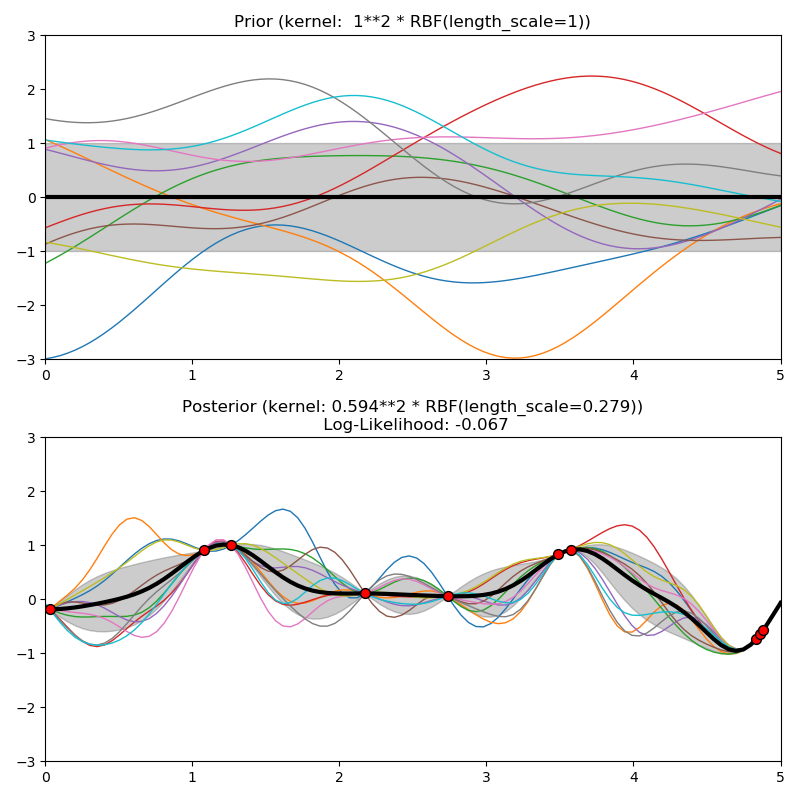
\includegraphics[width=0.7\linewidth]{sampleGP}
	\caption{Пример Гауссовского Процесса}
\end{figure}
Важным достоинством гауссовского процесса над другими моделями временных рядов являются его интерпретируемость, легкость имплементации и оценки. Что важно для приложения к задаче построения модели и учета априорных знаний, это интерпретируемость параметров. В ней главными являются значения среднего и магнитуды. В них можно учесть предположения о безусловном распределении доходностей алгоритмов.
\begin{align}
	f \sim \mathcal{GP}(m, k) \iff \E{f(x)} = m(x),\quad \E{(f(x) - m(x))(f(x')-m(x'))} = k(x, x'),
\end{align}
Где $m$ -- функция от $x$, но так же может быть и константой. Если считать, что доходности распределены по гаусовскому процессу, то параметр среднего можно интерпретировать, как среднюю доходность, магнитуду как средний риск. В работе будет рассмотрен гауссовский процесс с гауссовским ядром $k(x, x')=exp(-\tfrac{||x-x'||^2}{2\sigma^2})$.

Но в постановке GPVol, волатильность -- непостоянный параметр, этого можно добиться дополнительно введя шум на доходности, дисперсия которого подчиняется гауссовскому процессу.

\begin{align}
	r_m(t) & \sim GP_m\\
	r_v(t) & \sim GP_v\\
	r(t) & = r_m(t) + t_v(t)
\end{align}

\note{учет сдвига в моделях волатильности}
Волатильность -- косвенный показатель, и он не учитывается автором в явном виде. Поэтому процесс стохастической волатильности будем считать неизменным до и после структурного сдвига. Тем временем параметры среднего для процесса на средние доходности будут различаться <<до>> и <<после>> структурного сдвига.

\subsection{Моделирование динамики корреляций доходностей во времени}
\note{в чем сложность моделирования динамики корреляций?}
Моделирование динамики корреляций -- сложная задача, это скрытый марковский процесс с большим количеством скрытых состояний, квадратичным по количеству рядов. Без априорных предположений о структуре матрицы корреляций, вычислительная сложность слишком велика. Существует несколько основных подходов для моделирование динамики корреляций.
\begin{itemize}
	\item Dynamic Conditional Correlation (DCC) \citep{engle2000}
	\item Dynamic Equicorrelation Stochastic Volatility (DECO) \citep{kurose2016}
\end{itemize}
DCC модель моделирует динамику всей ковариационной матрицы, но не работает уже при хоть сколько нибудь значимой размерности. DECO модель берет свои истоки из DCC с дополнительной предпосылкой: существуют группы временных рядов, для которых парные корреляции одинаковы. Это позволяет снизить вычислительную сложность и уменьшить количество оцениваемых параметров.
\begin{align}
u_t &= \frac{\sum_{i\neq j} r_i r_j}{(n-1) \sum_{i} r_i^2}\\
\rho_{t+1} &= w + \alpha u_t + \beta \rho_t, \quad w/(1-\alpha-\beta) \in \left(\tfrac{-1}{n-1}, 1\right)
\end{align}
\note{что из этого можно использовать}
Сложность задания параметрической модели состоит в недостаточно подробном руководстве авторов статьи к имплементации. Более того, рекуррентные соотношения в вычислительном графе будут негативно сказываться на скорость вычислений. 
Естественным продолжением этой модели является гауссовский процесс для $\rho_t$ используя соответствующее  биективное преобразование $T:\: \mathbb{R} \to \left(\tfrac{-1}{n-1}, 1\right)$. Из-за гибкости и удобства моделирования этот метод и будет использован в итоговой спецификации.
На основании вышеизложенных причин, было решено использовать модификацию с гауссовским процессом, который не страдает от изложенных недостатков.

\begin{equation}
	\kappa_t = logit((\rho_t + \tfrac{1}{n-1} )/\tfrac{n}{n-1}))  \sim \mathcal{GP},
\end{equation}
где статистика $\kappa_t \in \Real$ и распределена согласно гауссовскому процессу. Такая параметризация крайне удобна, так как лишает необходимости задавать параметрический процесс. 

\section{Формирование модели динамики доходностей торговых стратегий: анализ различных спецификаций}
Объединяя части в одно целое, получим генеративную модель, учитывающую динамику корреляций торговых стратегий:
\paragraph{Расширенная спецификация с динамикой корреляций (DynCorr)}

\begin{align*}
\mu_\text{is} &\sim p(\mu_\text{is}); \in \Real^k& \text{ожидаемая доходность в обучающем периоде}\\
\mu_\text{oos} &\sim p(\mu_\text{oos});\in \Real^k&\text{ожидаемая доходность в тестовом периоде}\\
\nu &\sim p(\nu);\in \Real^k&\text{ожидаемый логарифм дисперсии}\\
\kappa &\sim p(\kappa);\in \Real& \text{ожидаемая статистика корреляции}\\
\theta_\mathcal{GP} &\sim p(\theta_\mathcal{GP})&\text{параметры многомерного гауссовского процесса}\\
\phi_\mathcal{GP} &\sim p(\phi_\mathcal{GP})&\\
\psi_\mathcal{GP} &\sim p(\psi_\mathcal{GP})&\\
\Delta\mu &\sim \mathcal{GP}(\theta_\mathcal{GP}); f:\Real \to \Real^k&\text{изменение доходности во времени}\\
\Delta\nu &\sim \mathcal{GP}(\phi_\mathcal{GP}); f:\Real \to \Real^k&\text{изменение логарифма дисперсии во времени}\\
\Delta\kappa &\sim \mathcal{GP}(\psi_\mathcal{GP}); f:\Real \to \Real&\text{изменение статистики корреляции во времени}\\
\end{align*}
\begin{align}
\mu_t &= \begin{cases}
\mu_\text{is} + \Delta\mu(t), t \in \text{\{обучающий период\}}\\
\mu_\text{oos} + \Delta\mu(t), t \in \text{\{тестовый период\}}
\end{cases}&\text{среднее доходностей в момент t}\nonumber\\
\sigma^2_t &= \exp(\nu + \Delta\nu(t))& \text{дисперсия доходностей в момент t}\nonumber\\
\rho_t &= \tfrac{k}{k-1}(\text{sigmoid}(\kappa + \Delta\kappa(t))-\tfrac{1}{k-1})&\text{корреляция доходностей в момент t}\nonumber\\
\Sigma_t &= ((1-\rho_t)\mathbb{I} + \rho_t) \odot \sigma_t\sigma_t^\top&\text{ковариационная матрица в момент t}\nonumber\\
R_t &\sim \mathcal{N}(\mu_t,\Sigma_t)& \text{наблюдаемые доходности в момент t}\label{eq:dyncorr}
\end{align}
где $k$ -- количество алгоритмов. Априорные распределения задаются исходя из природы данных и не могут быть указаны на этом этапе.

Априорные распределения играют важную роль в моделировании, их подбор субъективная задача. Она выполняется совместно с экспертами в области. В частности, большую поддержку оказали в Quantopian при проведении экспериментальной части. Благодаря экспертным знаниям получается учесть не только структурную составляющую зависимостей в модели, но также и априорные знания о параметрах. Это позволяет на малом наборе данных получать качественную модель, игнорировать выбросы, избегать эффекта переобучения. Так, априорное распределение на ожидаемые доходности формируется с учетом этапа селекции, который, как ожидается, отбирает наиболее стабильные алгоритмы из общей массы.

Обычной практикой является введение гипераприорного распределения -- арпиорное распределение на параметры априорного распределения. Оно позволяет сгладить возможно неудачный выбор фиксированных параметров априорного распределения и выражает неуверенность в изначальных предположениях. Эти подходы хорошо описаны например в \cite{daniel2014}. В этой работе гиперприоры -- широко используются еще и для моделирования некоторых других параметров, например стандартного отклонения для априорного распределения на средние доходности. Для упрощения выкладок гипераприорные распределения опущены в выкладках.

Несмотря на гибкость байесовского подхода остается проблематичным учесть неопределенность в структуре самой модели. Введение компоненты нестабильности корреляций во времени существенно усложняет модель как структурно, так и вычислительно. Гипотеза о необходимости динамики корреляций была сформирована на основании работ по рыночным активам \citep{vaga1990, oral2017}, подтверждается ли такое наблюдение на данных о доходностях алгоритмических стратегий -- вопрос, который подлежит изучению.

\note{Как тут использовать гауссовский процесс, как подбирать ядро}
Гауссовский процесс является центральной частью модели. Этот непараметрический метод, тем не менее, требует подбора ядра для каждой отдельной задачи. Временные ряды -- особый вид данных, часто требуется учитывать сезонность или тренд \citep{taylor2017}. Одним из бизнес процессов в компании является предварительный отбор алгоритмов, его проходят около 0.05\%. Успешно отобранные алгоритмы, что самое главное, имеют стационарное распределение доходностей. Таким образом, основной предпосылкой о структуре временного ряда будет его стационарность. Гауссовское ядро выражает вводимые предпосылки функционально, поэтому я буду использовать его в своей работе, более того, оно позволяет оптимизировать некоторые вычисления. 

Возможны альтернативные спецификации модели, которые учитывают не динамику корреляций, а наоборот, статику.
\note{переделать не списком, разжевать каждую спецификацию}
\paragraph{Спецификация со статическими корреляциями (Corr).}
Расширенная спецификация допускает упрощения. В случае, если не будет выявлено динамической корреляции в данных, осмысленно использовать спецификацию, которая вводит дополнительную предпосылку о неизменности корреляций. Более жесткие предпосылки не делают модель беднее. Напротив, предыдущая спецификация не позволяла иметь корреляции между подгруппами алгоритмов, и ковариационная матрица имеет блок диагональный вид. Эта же, напротив, позволяет оценивать полную ковариационную матрицу, хоть и постоянную во времени.
\begin{align}
L &\sim p(L);\in R^{k\times k}:\; L_{ii} > 0 & \text{нижняя треугольная матрица}\nonumber\\
\tilde{\Sigma} &= LL^\top & \text{<<средняя>> ковариационная матрица}\nonumber\\
\Sigma_t &= \tilde{\Sigma} \odot \sigma_t\sigma_t^\top & \text{ковариационная матрица в момент t}\label{eq:staticcorr}
\end{align}

Стоит отметить, что априорное распределение задается сразу в виде $p(\tilde{\Sigma})$, причем возможно одновременно контролировать как корреляции, так и дисперсии. Основным инструментом здесь является LKJ распределение \citep{lewandowski2009} на параметры корреляций. Оно позволяет контролировать число скоррелированных компонент: от диагональной ковариационной матрицы до плотной, где корреляций много. Это распределение рекомендовано использовать вместо Inverse Wishart \citep{haff1979}, которое не обладает хорошими свойствами интерпретируемости. 

Априорное распределение на дисперсии задается отдельно, как правило оно логнормальное, что и было использовано в данной работе. Альтернативой являются распределения с тяжелыми хвостами, как Half Cauchy или Half StudentT \citep{gelman2006scale}. 

\paragraph{Спецификация без корреляций (Diag).}
Принцип <<Бритвы Оккама>> -- лучше та модель, что максимально просто объясняет природу данных. Следуя этому принципы вводится в рассмотрение дополнительная спецификация, которая вообще исключает корреляции. Она более устойчива, проста в оценке. Не исключено, что более простая модель хорошо подойдет для практических задач.

\begin{equation}
\Sigma_t = diag(\sigma^2_t)\label{eq:nocorr}
\end{equation}

\note{Часть о достоинствах и недостатках спецификаций}
У каждой спецификации есть свои достоинства и недостатки. Так, даже расширенная спецификация \eqref{eq:dyncorr} в некоторых случаях может уступать более простой модели без динамики корреляций \eqref{eq:staticcorr}. Связано это с тем, что моделировать динамику полной ковариационной матрицы чрезвычайно трудная задача и приходится вводить предпосылку о структуре ковариационной матрицы. 

Вычислительные ресурсы, требуемые на оценку модели так же различаются. Модель \eqref{eq:staticcorr} слабо масштабируется по числу алгоритмов $k$, для которых производится оценка динамики, из-за требуемых объемов памяти: $\mathcal{O}(k^2)$ для хранения ковариационной матрицы. Модель учитывающая динамику корреляций избегает этой проблемы, однако требует большого количества вычислительных ресурсов.
\begin{table}[h]
	\caption{Сравнение спецификаций модели динамики доходностей финансовых стратегий по ключевым показателям}
	\begin{tabular}{l|c|c|c}
		& DynCorr \eqref{eq:dyncorr} & Corr \eqref{eq:staticcorr}& Diag \eqref{eq:nocorr} \\ \hline
		Динамика корреляций & $+$ & $-$ & $-$ \\ \hline
		Полная ковариационная матрица &$-$ & $+$ & $-$ \\ \hline
		Динамика волатильности  &$+$ & $+$ & $+$ \\ \hline
		Сложность оценки, ч. работы сервера &10 & 3 & $<1$ \\ \hline
		Масштабируемость по числу алгоритмов & Низкая & Средняя & Высокая
	\end{tabular}
\end{table}

Необходимая спецификация будет определяться исходя из предварительного эмпирического анализа. Итоговая модель, ее апостериорное распределение, будет оцениваться с помощью Markov Chain Monte Carlo метода NUTS \citep{hoffman2011nuts} семейства Hamiltonian Monte Carlo с имплементацией на языке \texttt{Python} в пакете PyMC3 \citep{salvatier2016pymc3}\footnote{К сожалению, из-за соглашения NDA, код проекта не публикуется}.

\paragraph{Hamiltonian Monte Carlo (HMC)} -- семейство методов, использующая информацию второго порядка (градиенты) для построения марковской цепи. Основной принцип заключается в использовании гимильтоновой динамики (понятие пришло из физики) чтобы получать симуляции из распределения, не имеющего нормализующей константы в явном виде. Обычно такая сложность возникает ввиду невозможности численного интегрирования по многим переменным.
\begin{equation}
p(x) \propto exp(-\tfrac{U(x)}{T})
\end{equation}
Модель представлена системой от позиции и скорости. Вместе они формируют энергию потенциальную и кинетическую:

\begin{equation}
E(x, v) = U(x) + K(v),\quad K(v)\sum_{i}\tfrac{mv^2}{2}
\end{equation}
Совместное же распределение $p(x, v)$ раскладывается на два независимых

\begin{equation}
p(x, v) \propto exp(-\tfrac{E(x, v)}{T}) = exp(-\tfrac{U(x)}{T})exp(-\tfrac{K(v)}{T})=p(x)p(v)
\end{equation}
Используя гамильтонову динамику мы можем сэмплировать из $p(x)$. Для этого необходимо сэмплировать $v \sim p(v)$, а далее, используя тождества из физики, преобразовать $x$ по следующей динамике:
\begin{equation}
\dot{x} = v,\quad m\dot{v} = \frac{\partial U(x)}{\partial x} \label{eq:hmctraj}
\end{equation}
Однако, используя исключительно динамику, так не получится по-настоящему сэмплировать из-за закона сохранения энергии. Поэтому траектории ограничены и скорость обновляется перед каждой симуляцией динамики. Но и тут не все гладко, необходимо проводить траектории \eqref{eq:hmctraj}, обычно используют leapfrog метод для этого.

\paragraph{No U-Turn Sampler (NUTS)} -- модификация обычного HMC, с поиском оптимальной длины интегрирования \eqref{eq:hmctraj}. На сегодняшний день он остается надежным методом, способным решать среднего размера задачи байесовского вывода. Существуют уже готовые реализации этого метода и ими удобно пользоваться \citep{salvatier2016pymc3}.

\paragraph{Альтернативные методы вывода}, например вариационные методы \citep{alp2015, jimenez2015, louizos2017}, вряд ли будут адекватно подходить под эту задачу, их основное преимущество состоит в том, что они работают в условиях большой размерности параметров и больших данных; это не наш случай. У нас данных мало и количество параметров не огромно. Более того, вариационные методы не всегда хорошо улавливают связи в распределении, что зачастую приводит к нежелательным последствиям. В работе не используются вариационные методы, поскольку основная рекомендация использовать HMC, пока он работает, иначе -- вариационные методы.
\section{Составление портфеля торговых стратегий на основе модели динамики доходностей}
Вероятностная модель задает распределение над возможными траекториями доходностей группы алгоритмов. С помощью байесовского вывода возможно оценить распределение на параметры, по реальным данным $p(\Theta\cond r_{1:T})$, после чего можно производить симуляции будущих траекторий 
\[r_{T+1:T'} \sim p(r_{T+1:T'}\cond r_{1:T}) = \int p(r_{T+1:T'}\cond\Theta, r_{1:T})p(\Theta\cond r_{1:T}) d\Theta\] 
Это позволяет учесть неопределенность реального поведения доходностей в будущем для формирования портфеля из торговых стратегий.

Используя выпуклую оптимизацию будем составлять портфель, который максимизирует изоэластичную функцию полезности:

\begin{minipage}{0.4\linewidth}
\begin{equation}
U_\rho(r) = \begin{cases}
\frac{r^{1-\rho}-1}{1-\rho}, &\rho\ne 1\\
\ln r, &\rho = 1
\end{cases}
\label{eq:isoelastic}
\end{equation}
\end{minipage}
\begin{minipage}{0.5\linewidth}
	\begin{figure}[H]
		\centering
		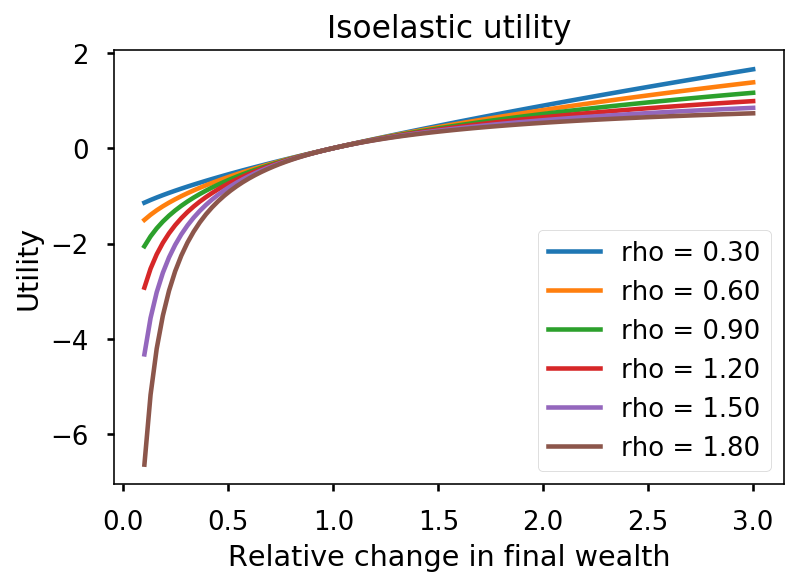
\includegraphics[width=0.7\linewidth]{Thesis/images/isoelastic}
		\caption{Изоэластичная функция полезности, При $\rho=0$ она риск нейтральна, при $\rho \to \infty$ достигается абсолютное избегание риска.}
		\label{fig:isoelastic}	
	\end{figure}
\end{minipage}
\vspace{.5cm}

 Для составления портфеля максимизируется  матожидание полезности. Выбранная функция обладает свойством избегания риска: потери учитываются в большей степени, чем выигрыши. Оптимальный портфель будет учитывать эти предпочтения.
\begin{align}
&r_{T+1:T'} \sim p(r_{T+1:T'}\cond r_{1:T})\\
&r^w = -1 + \prod_{t=T+1}^{T'} w^\top(r_t + 1)\\
&\Eb[r^w]{U_\rho(r^w)} \to \max_w, \quad w>0,\quad \sum w = 1
\end{align}
    % Вторая глава
\chapter{Практическое применение модели}
Понимание того, как будет работать модель на практике, важная часть исследовательской деятельности. На основе экспериментов можно будет давать практические рекомендации по подбору параметров, спецификации при использовании. Правильная постановка эксперимента позволит сравнить предложенный метод с бейзлайном.

\section{Описание данных}
\note{Этап создания алгоритмов}
Инфраструктура, созданная в компании, предусматривает взаимодействие с широким кругом лиц, которые внештатно создают торговые стратегии, получая за это небольшое вознаграждение. При написании алгоритма можно:
\begin{enumerate}
	\item выбрать торгуемые активы
	\item задать периодичность, с которой работает алгоритм
	\item собирать любые статистики с предыдущих периодов
	\item произвольным образом реструктурировать портфель основываясь на прошлой информации
\end{enumerate}
Обладая навыками программирования на \texttt{Python}, можно написать любую стратегию, которая использует только рыночные данные. Алгоритмов огромное количество, более 700 000, большинство из этих алгоритмов написаны энтузиастами. В отличие от рыночных активов, которых ограниченное количество, алгоримов гораздо больше. Это открывает широкие возможности для применения портфельной теории для создания диверсифицированного портфеля.

\note{Этап селекции алгоритмов}
Тем не менее, применять портфельную теорию проблематично. Для такого количества временных рядов длина ряда слишком мала. Расчет даже ковариационной матрицы требует огромных вычислительных мощностей и памяти. Для решения этой проблемы существует этап предварительного отбора алгоритмов, этап селекции. В инфраструктуре разработана модель, которая выбирает наиболее стабильные из совокупности\footnote{Детали реализации защищены NDA}. После этого этапа остается около 150 торговых стратегий, которые и были использованы для тестирования модели динамики.

\section{Проверка предпосылок и выбор спецификации модели}
Перед непосредственно оценкой спецификаций модели динамики доходностей, был проведен эмпирический анализ алгоритмов, отобранных после селекции. Основной его задачей было выяснить, какие предпосылки себя оправдывают и какая спецификация наиболее полно описывает распределение доходностей во времени. 

\begin{figure}[h]
	\centering
	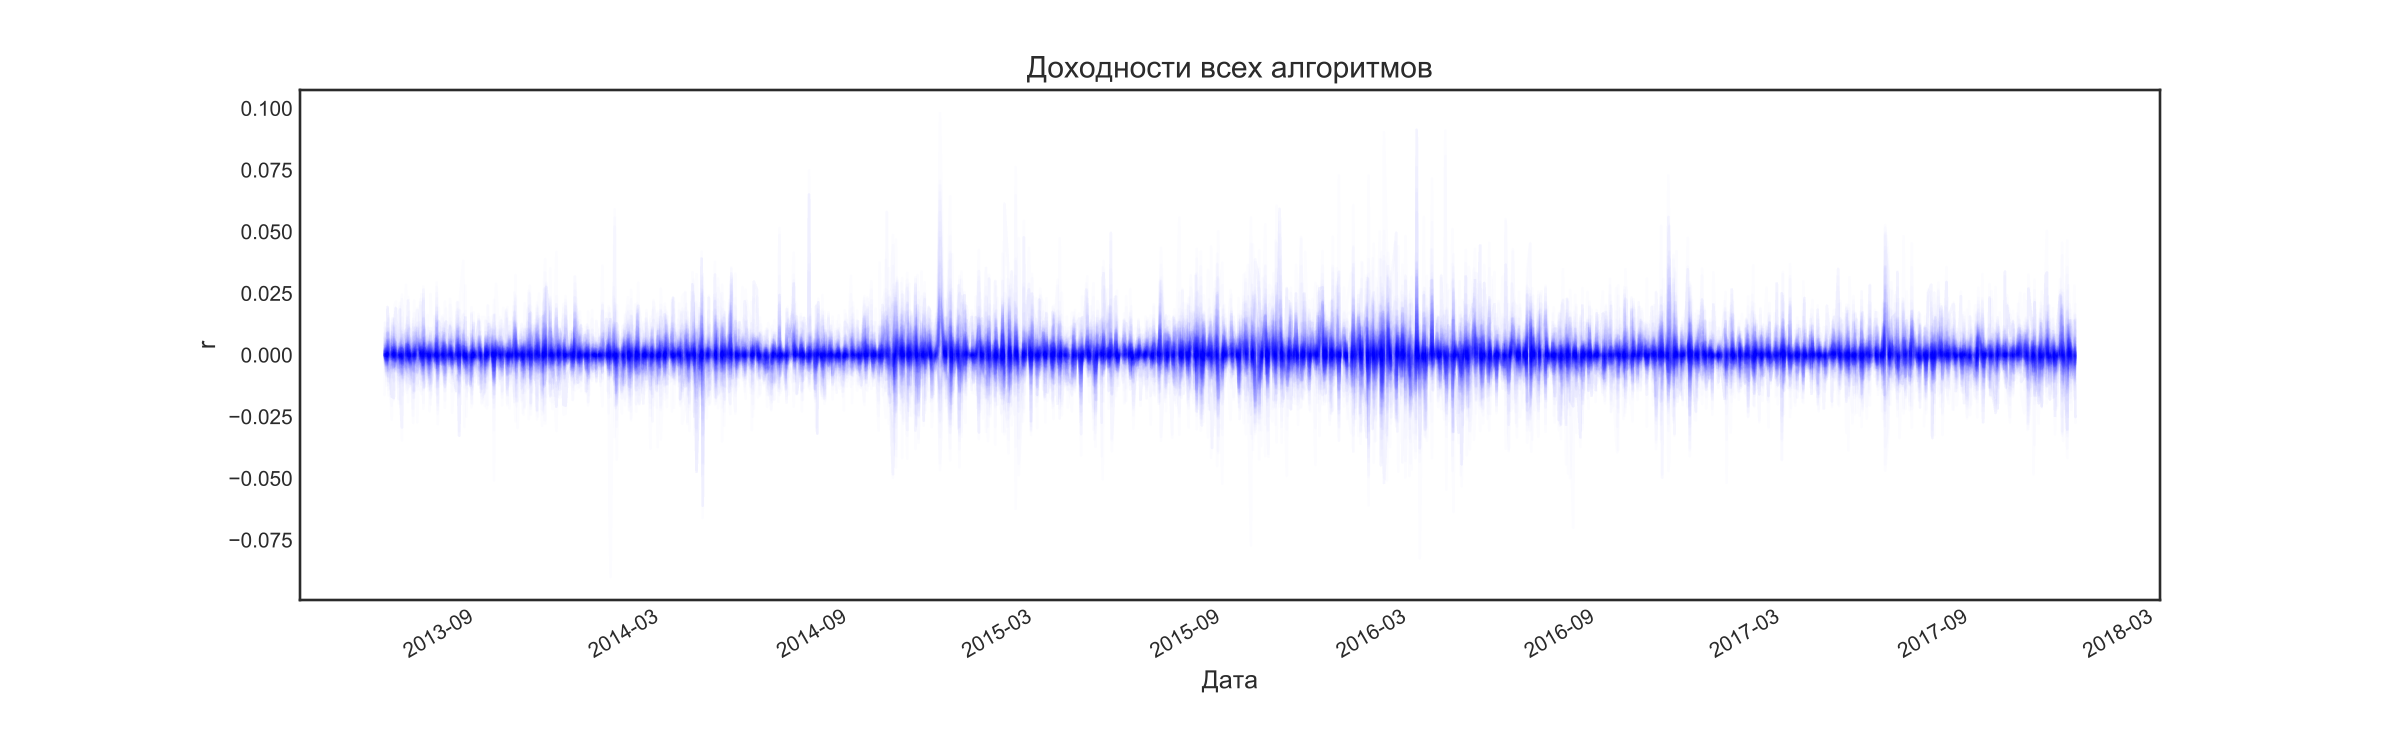
\includegraphics[width=\linewidth]{Thesis/images/returns-all.png}
	\caption{Доходности всех алгоритмов, на графике наблюдается непостоянная волатильность}
	\label{fig:allreturns}
\end{figure}

Гипотеза о непостоянстве волатильности находит свое подтверждение в графике распределения доходностей всех алгоритмов во времени (Рисунок \ref{fig:allreturns}). На нем видны периоды с высокой волатильностью. Более того, эффект наблюдается во многих алгоритмах в рамках одного периода.	

\begin{wrapfigure}{r}{.49\linewidth}
	\centering
	\includegraphics[width=\linewidth]{Thesis/images/returns-monthly}
	\caption{Распределение доходностей всех алгоритмов, сгруппированные по месяцам}
	\label{fig:monthlyreturns}
\end{wrapfigure}

Первичный анализ наличия сезонности в общем поведении алгоритмов не дал результатов: распределение доходностей, сгруппированных по месяцам выглядит однородно (Рисунок \ref{fig:monthlyreturns}).

\begin{figure}[h]
	\centering
	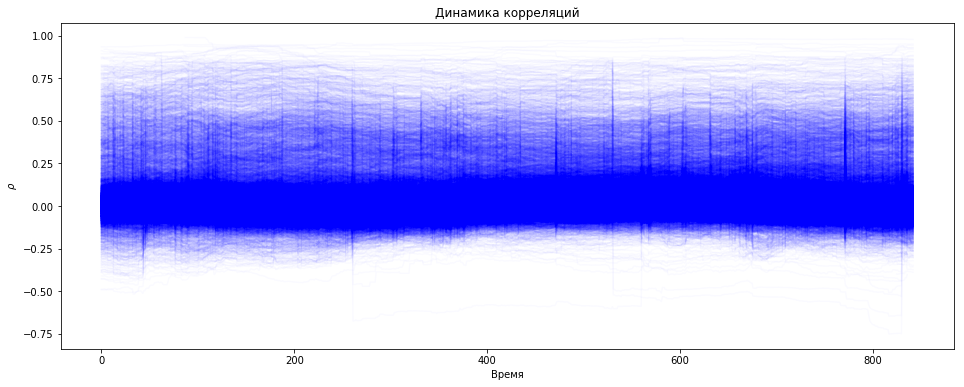
\includegraphics[width=\linewidth]{Thesis/images/correlations}
	\caption{График динамики корреляций между торговыми стратегиями. Попарные корреляции были посчитаны за период 2013-2017 с окном 300 дней. Не наблюдается существенного изменения корреляций за этот период.}
	\label{fig:correlations}
\end{figure}
Этап селекции имел важные последствия на спецификацию модели. Предположение о динамике корреляций оказалось не состоятельным (Рисунок \ref{fig:correlations})\footnote{Теста}. В данных не наблюдается существенного изменения корреляций для большой группы торговых стратегий. Значительное количество траекторий значительно отдалены от нуля. Тем не менее, на основе этого графика сделать вывод о структуре ковариационной матрицы (блочная/плотная) нельзя. В сложившейся ситуации этот анализ избыточен, так как семейство моделей с плотной матрицей ковариации включает в себя подмножество тех, что имеют блочную структуру. 

Выводы, которые можно сделать на основе проведенного анализа:
\begin{itemize}
	\item присутствует стохастическая волатильность
	\item сезонность в данных отсутствует или незначительна
	\item корреляции относительно стабильны во времени
	\item большинство корреляций околонулевые
\end{itemize}

Основываясь на них, остается сфокусироваться на двух спецификациях, которые не учитывают динамику корреляций:
\begin{itemize}
	\item модель без корреляций \eqref{eq:nocorr}
	\item модель со статичными корреляциями \eqref{eq:staticcorr}
\end{itemize}

Корреляционная матрица стабильна во времени, существуют негативные корреляции, много корреляций отличных от нуля, она имеет плотную структуру, которую невозможно учесть, используя блочной структуры матрицу. Модель, учитывающая динамику корреляций, не подходит для моделирования стохастического процесса доходностей торговых стратегий. Более того, в экспериментах модель страдала от ряда проблем:
\begin{itemize}
	\item Долгая фаза адаптации ковариационной матрицы <<пропозал>>\footnote{В английской литературе оно называется proposal distribution} распределения
	\item Долгая сходимость марковской цепи (более 10000 итераций)
	\item Продолжительные расчеты для оценки модели (около 12 ч.)
	\item Модель не работала для моделирования динамики большой группы алгоритмов
\end{itemize}

\section{Реализация моделей и сравнительный анализ в рамках портфельной оптимизации}
\note{Описание поставленного эксперимента}
Для качественных выводов о работе предложенного метода составления портфеля недостаточно оценить одну модель на подвыборке алгоритмов, так как это может быть случайный успех или неудача. Для проведения эксперимента на реальных данных, был использован метод бутстрап \citep{grimshaw1995} и разделение выборки на обучающую и тестовую.

\textbf{Постановка эксперимента:}
\begin{itemize}
	\item Всего 4 года наблюдений
	\item Обучающая выборка -- первые два года
	\item Тестовая выборка -- последние два года
	\item Сгенерировано 400 выборок алгоритмов размера 20 из 150 без повторений
	\item Тремя методами: предложенными \eqref{eq:staticcorr}, \eqref{eq:nocorr} и по Марковицу, строятся портфели основываясь на данных обучающей выборки
	\item Считается критерий качества (коэффициент Шарпа) на тестовой выборке
\end{itemize}

\note{Параметры NUTS}
Для оценки апостериорных распределений параметров модели использовался алгоритм NUTS \citep{hoffman2011nuts}, при этом генерировалась выборка размера 3000 из этого распределения. Для оценки потребовались большие вычислительные мощности. Так, расчет модели на динамику 20-ти алгоритмов со статическими корреляциями \eqref{eq:staticcorr} занимает около 3х часов на 32х-ядерном сервере. Оценка модели без корреляций \eqref{eq:nocorr} занимает менее получаса. Весь эксперимент длился более месяца.

\note{Описание и трактовка результатов}
Результаты эксперимента предствлены на на рисунке \ref{fig:performance}. На первой строчке изображены распределения коэффициентов Шарпа, получаемые разными методами: методом Марковица (Mark, всегда черным цветом), через модель со статическими корреляциями (Corr) и без корреляций (Diag) соответственно. На второй строчке изображены распределения разности коэффициентов Шарпа полученных с помощью модели Corr и Diag, Corr и Mark, Diag и Mark. На третьей строчке изображена разность волатильности портфеля для Corr и Diag и далее плотности волатильности моделей Corr, Diag и Mark. Цветовая шкала означает значение параметра $\rho$ в функции полезности \eqref{eq:isoelastic}. Распределение коэффициента Шарпа на тестовом периоде находится значительно правее, что означает преимущество предложенного метода над ранее используемым аналогом. 

Из экспериментов следует, что предложенный алгоритм более устойчив при обучении, обладает необходимой обобщающей способностью для улучшения качества портфеля по ряду показателей. В целом не важно, какую спецификацию модели выбирать: дополнительное моделирование корреляций не принесло большой пользы, разница волатильности и коэффициентов Шарпа между моделью \eqref{eq:staticcorr} и \eqref{eq:nocorr} имеет сконцентрированное в нуле распределение.
\begin{figure}[h]
	\centering
	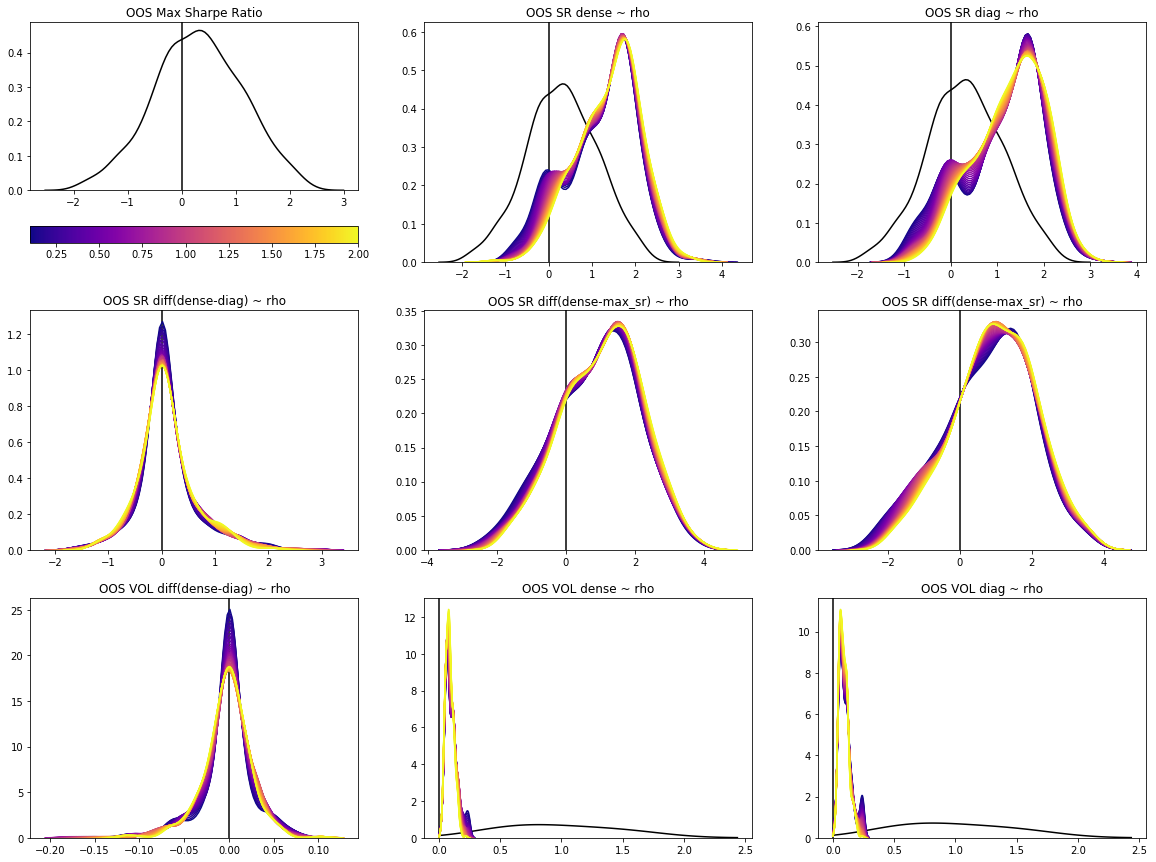
\includegraphics[width=\linewidth]{Thesis/images/performance}
	\caption{Сравнение коэффициента Шарпа на тестовой выборке байесовского (выделен цветом) и оптимального портфеля Марковица (черным) полученного методом бутстрап. Распределение коэффициента Шарпа на тестовом периоде находится значительно правее, что означает преимущество предложенного метода над ранее используемым аналогом. }
	\label{fig:performance}
\end{figure}
\\\\
\textbf{Основные выводы}
\begin{itemize}
	\item Коэффициент Шарпа: в 70\% случайно выбранных портфелях коэффициент Шарпа больше полученного методом Марковица
	\item Дисперсия получаемого портфеля новым способом ниже
	\item Моделирование корреляций не дает существенного преимущества перед моделью без них
\end{itemize}

   % Третья глава
\chapter*{Заключение}
\addcontentsline{toc}{chapter}{Заключение}

В ходе проведенного исследования решены следующие задачи:
\begin{enumerate}
	\item Предложена общая схема моделирования динамики торговых стратегий, которая учитывает особенности, связанные с их доходностями. Результаты исследования включают в себя реализацию трех спецификаций модели с учетом, без учета динамики корреляций и упрощенная -- без корреляций. Для оценки модели динамики корреляций предложена модификация базового метода DECO с использованием гауссовского процесса

	\item Все три спецификации модели динамики доходностей торговых стратегий реализованы на языке \texttt{Python} с использованием специализированных библиотек для байесовского моделирования
	
	\item Реализована процедура составления портфеля торговых стратегий методом монте--карло

	\item Проведенный эмпирический анализ позволил сделать вывод о непостоянстве волатильности и постоянстве корреляций доходностей торговых стратегий

	\item С помощью сравнения методом бутстрап показана практическая значимость предложенного подхода для использования его в качестве инструмента для составления портфеля торговых стратегий. Портфель, основанный на предложенной модели оказывается эффективнее модели Марковица по ряду критериев (имеет большую обобщающую способность, более высокий коэффициент Шарпа на экзаменационной выборке). Предложенная позволяет получить более устойчивый во времени портфель.
\end{enumerate}

Проведенное исследование подтверждает целесообразность использования байесовских методов в формировании портфеля торговых стратегий. Такой подход позволяет учесть априорные знания о модели. Портфель, построенный на симуляциях из нее, получается более устойчивым во времени и, как следствие, более доходным на экзаменационном периоде.

      % Заключение
\clearpage                                  % В том числе гарантирует, что список литературы в оглавлении будет с правильным номером страницы
%\hypersetup{ urlcolor=black }               % Ссылки делаем чёрными
%\providecommand*{\BibDash}{}                % В стилях ugost2008 отключаем использование тире как разделителя 
\urlstyle{rm}                               % ссылки URL обычным шрифтом
\ifdefmacro{\microtypesetup}{\microtypesetup{protrusion=false}}{} % не рекомендуется применять пакет микротипографики к автоматически генерируемому списку литературы
\bibliography{biblio/cites}
\bibliographystyle{BibTeXStyles/iclr2018workshop}
\ifdefmacro{\microtypesetup}{\microtypesetup{protrusion=true}}{}
\urlstyle{tt}                               % возвращаем установки шрифта ссылок URL
%\hypersetup{ urlcolor={urlcolor} }          % Восстанавливаем цвет ссылок      % Список литературы
\appendix
%%% Оформление заголовков приложений ближе к ГОСТ:
\setlength{\midchapskip}{20pt}
\renewcommand*{\afterchapternum}{\par\nobreak\vskip \midchapskip}
\renewcommand\thechapter{\Asbuk{chapter}} % Чтобы приложения русскими буквами нумеровались
   % Предварительные настройки для правильного подключения Приложений
        % Приложения

\end{document}
